
\begin{abstract}[\hspace*{-10pt}]
    This chapter draws mainly on the submitted work: \fullcite{van_biesbroeck_generalized_2024}  % Ce chapitre reprend principalement les travaux publiés dans: 
\end{abstract}

\begin{abstract}
    This chapter complements the reference prior theory. We propose an interpretation of the theory from a sensitivity analysis viewpoint. This leads us to propose a new way of defining mutual information, using different dissimilarity measures between probability distributions. 
    Our construction  creates a new framework for reference priors, which are rigorously studied.
    Our main result gives a limit of the generalized mutual information when the dissimilarity measure considered resembles to a $\delta$-divergence.
    It makes it easier to derive reference priors under constraints or within specific sets. In the absence of constraints, we prove that the Jeffreys prior maximizes the generalized mutual information, reinforcing its objective characteristic.
\end{abstract}

\minitoc

\section{Introduction and motivations}

The reference prior theory aims at defining priors that are the most objective possible. A review of the theory can be found in the \cref{chap:intro-ref}. It is built on the maximization of the mutual information, which is designed to measure the information brought by the data in the posterior distribution.

Although there are infinite ways % exist infinitely many ways 
to compare probability distributions, the mutual information is classically defined as an expected Kullback-Leibler divergence between the prior and the posterior.
The settings under which the reference priors are usually defined result from the aforementioned choice. Since the aim is to define priors that are not impacted by potentially subjective choice, we ask how the results about reference priors change when the definition of the mutual information is modified.
% question how the results about reference priors stands when the definition of the mutual information is altered.

Extensions of the mutual information in the reference prior definition have already been explored in the literature (e.g. \cite{chen_objective_2010,liu_divergence_2014,le_formal_2014}), and some do not necessarily lead to the Jeffreys prior \citep{hashimoto_reference_2021,clarke_reference_1997,ghosh_general_2011}. They are all based on the expression of mutual information as an average divergence between the posterior and the prior distributions.




In this chapter, we contribute to the reference prior theory with an original derivation of the mutual information from a Global Sensitivity Analysis (GSA) based viewpoint. %that we divulge.
GSA, whose principle is to measure how the uncertainty of an output is impacted by that of some of its input \citep{iooss_review_2015}, allows us indeed to provide %indeed
an interpretation of the reference prior as a maximizer of such sensitivity influence that the observations get from the parameter of interest. 
This suggestion leads to defining what we call generalized mutual information, by analogy with global sensitivity indices (which are introduced for instance in \cite{da_veiga_basics_2021}). %
It relies on the wide range of existing dissimilarity measures between two probability distributions.
An example is the $f$-divergence subclass \citep{csiszar_information-type_1967}, commonly employed as an extension of  Shannon's entropy for various purposes in statistics, such as, variational inference \citep{minka_divergence_2005,bach_sum--squares_2023}, surrogate model design \citep{nguyen_surrogate_2009}, PAC Bayesian learning \citep{picard-weibel_change_2022} and Differential Privacy \citep{mironov_renyi_2017}.
%
A study of those divergences within our generalized mutual information is {also} a main contribution of this chapter, with the goal of deriving what one is invited to call generalized reference priors.
%Pursuing introductory elements we unveiled in \cite{VanBiesbroeckJDS2023}, we go further in this paper with 
We provide an accomplished formalization for the generalized reference prior settings, and results based on classical $f$-divergences for sensitivity analysis such as $\delta$-divergences.
{
Our main result takes the form of a limit w.r.t. the number of data of the mutual information. Its analytical expression as a function of the prior permits a simple expression of our reference priors: they are its maximal arguments. It opens the path of easier {theoretical} derivation of reference priors among the ones that satisfy different kinds of constraints, or that belong to some particular sets of priors.}


In the next section, %we formalize the usual Bayesian framework that we consider in our work. 
we elucidate our motivation 
from a Global Sensitivity Analysis viewpoint for an enrichment of the mutual information. 
The generalized mutual information that we define is constructed from any possible dissimilarity measure.
That definition is used in \cref{sec:PSGSA:generefp} to define the generalized reference priors. We show in that section that the usual properties satisfied by reference priors still stand under our framework.
A deeper study is afterward conducted in \cref{sec:PSGSA:towardsdelta} in the case where the dissimilarity measure is an $f$-divergence resembling to a $\delta$-divergence. 
These results, alongside open thoughts about their robustness when the dissimilarity measure is not limited to such $f$-divergences, are discussed in \cref{sec:PSGSA:discussion}.
After proving our statements in \cref{sec:PSGSA:proofs}, we conclude this chapter in \cref{sec:PSGSA:conclusion}.







\section{Generalized mutual information}\label{sec:PSGSA:genMI}

\subsection{Mutual information and definitions}


We consider a statistical modeling characterized by a collection of distributions $(\PP_{Y|\theta})_{\theta\in\Theta}$. 
The Bayesian framework is constructed as described in the \cref{chap:intro-ref} (\cref{sec:intro-refs:limits}). We suppose that $\Theta\subset\RR^d$ and denote by $\nu$ the Lebesgue measure on $\RR^d$. 
The priors considered are absolutely continuous distributions w.r.t. $\nu$.

We consider the same notations as in \cref{chap:intro-ref}: $\mbf Y_k$ denote a random vector of $k$ data items whose distribution conditionally to $T=\theta$ is $\PP_{\mbf Y_k|\theta}:=\PP_{Y|\theta}^{\otimes k}$, where $T$ is an r.v. whose distribution is the prior $\varPi$ (which is not necessarily a probability distribution, see \cref{sec:intro-ref:novelframework}). The density of $\varPi$ is denoted by $\pi$.

We suppose that the modeling admits a likelihood, denoted by $\ell$ with $\forall\theta\in\Theta,\mbf y\in\cY^k,\, \ell_k(\mbf y|\theta)=\prod_{i=1}^k\ell(y_i|\theta) $. For all $\theta$, $\ell(\cdot|\theta)$ is the density of $\PP_{T|\theta}$ w.r.t. a common measure $\mu$ on $\cY$. We denote by $p_{\mbf Y^k}$ the marginal density of $\mbf Y_k$, and by $p(\cdot|\mbf y)$ the posterior density given the observations $\mbf y\in\cY^k$. %We recall that even though those quantities are defined (when they exist) only up to a constant, their definition is the usual o
Furthermore, we suppose the modeling to be regular (i.e. \cref{assu:intro-ref:jeffreysexist} in \cref{chap:intro-ref} is verified), so that the Fisher information matrix (that we denote $\cI$) and the Jeffreys prior exist. A density of the Jeffreys prior is denoted by $J$.



Under this framework, when the prior $\varPi$ is proper, %and its total mass equals $1$, 
we recall that the mutual information is classically defined as the following quantity:
    \begin{equation}\label{eq:PS:MI1orig}
        \sI^k(\varPi) =  \EE_{\mbf Y_k\sim \PP_{\mbf Y_k}}[\text{KL}(\PP_{T|\mbf Y_k}||\varPi)] .
    \end{equation}
We recall that in the above expression, the posterior and marginal distributions depend on the prior considered. %We do not write explicitly the dependance in the equations to avoid notations that are hard to read.
Applying Fubini-Lebesgue's theorem allows to also write the mutual information as follows
    \begin{equation}\label{eq:PS:MIGSA}
        \sI^k(\varPi) = \EE_{T\sim\varPi}[\text{KL}(\PP_{\mbf Y_k|T}||\PP_{\mbf Y_k}) ].
    \end{equation}
That last quantity expresses the mutual information as 
a measure of the influence that the stochastic parameter $T$ has on the data $\mbf Y_k$.
That interpretation aligns with a sensitivity analysis viewpoint. Actually, the expression in \cref{eq:PS:MIGSA} can be seen as a sensitivity index, where the impact of the input $T$ on the output $\mbf Y_k$ is studied. We develop this interpretation in the following section.

%\textcolor{orange}{proof of the funbini}

\begin{proof}[Proof that \cref{eq:PS:MI1orig} and \cref{eq:PS:MIGSA} are  equal]
    One can remark that for any $x\in(1,\infty)$, $|\log x|\leq x-\log x$. That statement allows applying \cref{prop:PS:invertibility}, which is stated later on, with $f=-\log$. It provides the desired equality whether the involved quantities are finite or infinite.
    %One can prove that the quantities are finit
    % We wdefine $f(x)=-\log x$
\end{proof}



\subsection{Mutual information as a sensitivity index}

The integration of the Bayesian formalism in the settings of uncertainty quantification resorts in modeling $\mbf Y_k$ as the output of a stochastic system whose inputs include $T$. In other terms, we write $\mbf Y_k=\cM(T,\epsilon)$. Here, $T$ embeds uncertainty on  the input parameters and $\epsilon$ represents an unknown uncertain variable, sometimes referred to as a nuisance parameter.

A well-designed Bayesian modeling parameterized by $T$ would be such that the input between $\epsilon$ and $T$ whose impact on the output
is the highest is $T$. Such a modeling should reduce the impact of the irreducible uncertainty embedded in $\epsilon$.

This impact is measured by a sensitivity index as follows, considering a dissimilarity measure $D$, 
    \begin{equation}
        S = \EE_{T\sim\varPi}[ D(\PP_{\mbf Y_k}||\PP_{\mbf Y_k|T}) ].
    \end{equation}
It corresponds to the mutual information $\sI^k(\varPi)$ when $D$ is defined as $D(P||Q)=\text{KL}(Q||P)$.

Actually, different choices for dissimilarity measures $D$ can be done to define sensitivity indices \citep{da_veiga_global_2015}. For instance, setting $D(P||Q)=|\EE_{X\sim P}X-\EE_{X\sim Q}X|^2$ gives the un-normalized Sobol’ index \citep{sobol_sensitivity_1993}.
Among the most common ones, we recall the $f$-divergences, defined from a real and measurable function $f$ that is convex and maps $1$ to $0$. The $f$-divergence is denoted $D_f$ and defined as 
    \begin{equation}
        D_f(P||Q) = \int_\cX f\left(\frac{p(x)}{q(x)}\right) q(x) d\omega(x)
    \end{equation}
where $p,q$ respectively are densities of $P$ and $Q$  w.r.t. a common measure $\omega$ on $\cX$.







\subsection{Generalized mutual information definition}


The same way as sensitivity indices are supported by various dissimilarity measures, our suggestion is to define the mutual information using other dissimilarity measures than the Kullback-Leibler divergence.
Our novel definition is the following.
\begin{defi}[$D$-mutual inforamation]
    Let $D$ be a dissimilarity measure, for a fixed $k$, the $D$-mutual information of a proper prior $\varPi$ with total mass equal to $1$ under $k$ observations is defined as
        \begin{equation}
            \sI_D^k(\varPi) := \EE_{T\sim\varPi}[D(\PP_{\mbf Y_k}||\PP_{\mbf Y_k|T} )].
        \end{equation}
\end{defi}

In the case where $D=D_f$ is an $f$-divergence, the mutual information equals
    \begin{equation}
        \sI_{D_f}^k(\varPi) =\EE_{T\sim\pi}[D_f(\PP_{\mbf Y_k}||\PP_{\mbf Y_k|T})] = \int_\Theta\int_{\cY^k}f\left( \frac{p_{\mbf Y_k}(\mbf y)}{\ell_k(\mbf y|\theta)} \right) \ell_k(\mbf y|\theta)d\mu^{\otimes k}(\mbf y) \pi(\theta)d\theta.
    \end{equation}
% For the sequel, let us refer to the $D_f$-mutual  information as the $f$
It corresponds to  the classical definition in the case where $f=-\log$. Actually, the classical definition is a subcase of the study of a particular class of the $f$-divergences:  the $\delta$-divergences. They are defined setting $f=f_\delta$ where 
\begin{equation}
    f_\delta(x) = \left\lbrace\begin{array}{l l} \frac{x^\delta-\delta x-(1-\delta)}{\delta(\delta-1)} & \text{if\ }\delta\not\in\{0,1\},\\ 
        x\log x-x+1  & \text{if\ }\delta=1, \\
        -\log x +x -1 & \text{if\ }\delta=0.
    \end{array}\right. 
\end{equation}    
When $\delta=0$, we retrieve the original form (KL form) of the mutual information.


\section{Generalized reference priors}\label{sec:PSGSA:generefp}

%\subsection{Definitions and general properties}

Reference priors are defined as asymptotic maximizers of the mutual information. Using the same formalism as in their original definition (that is expressed in the \cref{chap:intro-ref}), we suggest the following definition of generalized reference priors using our generalized mutual information.

\begin{defi}[Generalized reference prior]\label{def:genref}
    Let $D$ be a dissimilarity measure and $\cP$ a set of priors on $\Theta$. A prior $\varPi\in\cP$ is called a $D$-reference prior over $\cP$ with rate $\varphi(k)$ if there exists an openly increasing  sequence of compact subsets $(\Theta_i)_{i\in\NN}$
    such that $\bigcup_{i\in\NN}\Theta_i=\Theta$ and for any $i$: $0<\varPi(\Theta_i)<\infty $ and
    % with $\pi^\ast(\Theta_i)>0$, $\Theta_i\subset\Theta$, $\bigcup_{i\in I}\Theta_i=\Theta$ such that
        \begin{equation}\label{eq:defrefpriorsi}
            \lim_{k\rightarrow\infty}\varphi(k)[\sI^k_D(\varPi(\cdot|\Theta_i))-\sI^k_D(P(\cdot|\Theta_i))] \geq0 \text{\ for all\ } P\in\cP\text{\ verifying\ }0<P(\Theta_i)<\infty;
        \end{equation}
    where  $\varphi(k)$ is a {positive and}  monotonous function of $k$.
\end{defi}
%In such defintion inv


This definition matches with the original one when the dissimilarity measure is the Kullback-Leibler divergence. Nevertheless, it introduces the definition of an associated rate proposed by ourselves. In fact, our
work provides elements showing that such rate exists and may vary as a function of the dissimilarity measure
considered.
The idea behind $\varphi$ is to look for an asymptotic expansion of $\sI^k_D(P_1)-\sI^k_D(P_2)$ that stands for any tuple of probability distributions $(P_1,P_2)$:
    \begin{equation}
        \sI^k_D(P_1)-\sI^k_D(P_2) \aseq{k\rightarrow\infty} \varphi(k)(L(P_1)-L(P_2)) + o(\varphi(k)),
    \end{equation}
where $L$ is a mapping that does not depend on $P_1$ or $P_2$.
%appropriate rate is given by $\varphi$ such that that
%$\sI^k(P_1)$
When it resorts to the original mutual information, the rate $\varphi$ is constant.

The results provided below ensure that the generalized reference priors verify similar properties as the original reference priors.







\begin{prop}[Invariance by reparametrization]
    Consider a reparametrization $\phi=g(\theta)$ with $g$ being a diffeomorphism and $\cP$ a set of priors on $\Theta$.
    Then if $\varPi$ is  a reference prior over $\cP$ for the model parameterized by $\theta$, $\tilde{\varPi}$ is a reference prior over $\tilde\cP$ for the model parameterized by $\phi$, where: 
    \begin{equation}
        \tilde\cP = \{ M(\pi |\det g_\phi^{-1}|),\,M(\pi)\in\cP ) \},
    \end{equation}
    with $M:f\in\sR\longmapsto (B\mapsto\int_B f(\theta)d\theta)\in\sM^\nu$. %mapping a function to the distribution whose it is the density.
\end{prop}

\begin{proof}
    The proposition comes from the fact that $\sI^k_D$ is
    clearly invariant by reparametrization: for any prior $\varPi$ having a density $\pi$ on $\Theta$, and any $\tilde\Theta\subset\Theta$ with $\varPi(\tilde\Theta)\in(0,\infty)$, calling $\tilde\Xi = g(\tilde\Theta) $,
        \begin{equation}
            \sI^k_D(\varPi(\cdot|\tilde\Theta)) = \EE_{T\sim\varPi(\cdot|\tilde\Theta)}[D(\PP_{\mbf Y_k}||\PP_{\mbf Y_k|T} )] = \EE_{\Phi\sim\tilde\varPi(\cdot|\tilde\Xi)} [D(\PP_{\mbf Y_k}||\PP_{\mbf Y_k|g^{-1}(\Phi)} )] =: \tilde\sI^k_D(\tilde\varPi(\cdot|\tilde\Xi))
        \end{equation}
    where $\tilde\varPi$ is defined by its density $\tilde\pi = \pi|\det d_\phi g^{-1}|$, and $\tilde\sI^k_D$ denoted the $D$-mutual information on the reparameterized model.
\end{proof}

\begin{prop}[Consistency with compact cases]
    Assume $\Theta$ is compact. Let $\cP$ be a set of continuous priors. If $\varPi$ is a reference prior over $\cP$ with rate $\varphi$, then
        \begin{equation}
            \lim_{k\rightarrow\infty} \varphi(k)[ \sI_D^k(\varPi) -\sI_D^k(P)] \geq0 \text{\ for all\ } P\in\cP.
        \end{equation}
\end{prop}

\begin{proof}
    As the priors are continuous, their restrictions are proper on any compact. Thus, the quantities involved in the proposition are well-defined. 
    As $\varPi$ is a reference prior over $\cP$ we can consider an associated openly increasing sequence of compacts $(\Theta_i)_{i\in\NN}$ that covers $\Theta$. Since $\Theta$ is compact there exists $i$ such that $\Theta_i=\Theta$. Hence the result since the renormalized restriction $\varPi(\cdot|\Theta_i)$ verifies the statement of the proposition by definition.
\end{proof}

\begin{prop}[Invertibility]\label{prop:PS:invertibility}
    %We consider an $f$-divergence $D_f$. If $\varPi$ admits a density $\pi$ which is such that for any compact set $\tilde\Theta$,
    Consider that $\varPi$ is a continuous prior and let $f$ be a convex function. %that $f$ is a convex function such that %$x\mapsto f(1/x)$ is concave 
    % for any compact set $\tilde\Theta$,
    \begin{enumerate}
        \item If for a compact set $\tilde\Theta$,
        \begin{equation}
            \sup_{\theta\in\tilde\Theta}\sup_{\theta'\in\tilde\Theta} \int_{\cY^k} f\left(\frac{\ell_k(\mbf y|\theta')}{\ell_k(\mbf y|\theta)}  \right) \ell_k(\mbf y|\theta) d\mu^{\otimes k}(\mbf y)<\infty
        \end{equation}
    Then the $D_f$-mutual information value of $\varPi(\cdot|\tilde\Theta)$ is finite. %restricted to compacts are always finite. 
        \item
    If there exist $K\geq0$ such that for any $x>0$, $|f(x)\indic_{f(x)<0}|\leq Kx $ then the $D_f$-mutual information restricted to compact expression can be inverted back:
        \begin{equation}\label{eq:PS:fubDf}
            \EE_{T\sim\varPi(\cdot|\tilde\Theta)}[D_f(\PP_{\mbf Y_k}||\PP_{\mbf Y_k|T})] 
                =\EE_{\mbf Y_k\sim\PP_{\mbf Y_k}} [D(\varPi(\cdot|\tilde\Theta)|| \PP_{T|\mbf Y_k} ) ]. 
        \end{equation}
    \end{enumerate}
\end{prop}

\begin{proof}
    %Let $\tilde\Theta$ be a compact subset of $\Theta$. We consider $\varPi\in\sM^\nu$ 
    We denote $\tilde\varPi=\varPi(\cdot|\tilde\Theta)$ and  $\tilde\pi$ the latter's density. We have
        \begin{equation}
        \begin{aligned}
            \sI^k_{D_f}(\tilde\varPi) &= \int_{\tilde\Theta}\int_{\cY^k} f\left( \frac{p_{\mbf Y^k}(\mbf y)}{\ell_k(\mbf y|\theta)}\right)\ell_k(\mbf y|\theta) d\mu^{\otimes k}(\mbf y) \tilde\pi(\theta)d\theta \\
                &\leq \sup_{\theta\in\tilde\Theta}\int_{\cY^k} \int_{\tilde\Theta} f\left( \frac{\ell_k(\mbf y|\theta')}{\ell_k(\mbf y|\theta)}\right)\ell_k(\mbf y|\theta) \tilde\pi(\theta')d\theta' d\mu^{\otimes k}(\mbf y) ,
        \end{aligned}
        \end{equation}
        using the convexity of $f$. Since $\tilde\Theta$ is compact, $\tilde\pi$ is bounded. Thus, we obtain $\sI^k_{D_f}(\tilde\varPi)<\infty$.

        For inverting the integrals, we notice that the assumption on $f$ allows writing 
        \begin{equation}\label{eq:PS:prooffub1Dfbound}
            \int_{\tilde\Theta}\int_{\cY^k} \left|f\left( \frac{p_{\mbf Y^k}(\mbf y)}{\ell_k(\mbf y|\theta)}\right)\right|\ell_k(\mbf y|\theta) d\mu^{\otimes k}(\mbf y) \tilde\pi(\theta)d\theta \leq 2K + %\sup_{\theta\in\tilde\Theta}\sup_{\theta'\in\tilde\Theta} \int_{A} f\left(\frac{\ell_k(\mbf y|\theta')}{\ell_k(\mbf y|\theta)}  \right) \ell_k(\mbf y|\theta) d\mu^{\otimes k}(\mbf y)
            \int_{\tilde\Theta}\int_{\cY^k} f\left(\frac{p_{\mbf Y_k}(\mbf y)}{\ell_k(\mbf y|\theta)}\right)\ell_k(\mbf y|\theta)d\mu^{\otimes k}(\mbf y)\tilde\pi(\theta)d\theta %= 2K+ \sI^k_{D_f}(\tilde\varPi)
        \end{equation}
        using $|f(x)|\leq 2Kx\indic_{f(x)<0}+f(x)$.
        %using $|\log x|\leq\log x + x^{-1}\indic_{x<1}$
        %with $A=\{\mbf y\in\cY^k,\, p_{\mbf Y_k}(\mbf y)/\ell_k(\mbf y|\theta)\in f^{-1}((0,\infty)) \}\subset\cY^k $. 
        We deduce that, if $\EE_{T\sim\tilde\varPi}[D_f(\PP_{\mbf Y_k}||\PP_{\mbf Y_k|T})]$ is finite, then Fubini-Lebesgue's theorem can be applied, leading to the equality \eqref{eq:PS:fubDf}.
        The same way, we have
        \begin{equation}
            \int_{\cY^k} \int_{\tilde\Theta} \left|f\left( \frac{\tilde\pi(\theta)}{p(\theta|\mbf y)}\right)\right|p(\theta|\mbf y)d\theta p_{\mbf Y_k}(\mbf y) d\mu^{\otimes k}(\mbf y) 
            \leq 2K + \int_{\cY^k}\int_{\tilde\Theta}f\left( \frac{\tilde\pi(\theta)}{p(\theta|\mbf y)}\right) p(\theta|\mbf y)d\theta p_{\mbf Y_k}(\mbf y) d\mu^{\otimes k}(\mbf y),
        \end{equation} 
        so that if $\EE_{\mbf Y_k\sim\PP_{\mbf Y_k}}[D_f(\tilde\varPi||\PP_{T|\mbf Y_k})]$ is finite, the integrals can also be inverted and equality \eqref{eq:PS:fubDf} still stands.
        We conclude by deducing that, if one of the quantity in \cref{eq:PS:fubDf} is infinite, the other cannot be finite, letting the equality to stand as well.
        %
        %the above quantity is finite, which allows us to invert the integrals and conclude, using Fubini-Lebesgue's theorem.
        %
        %Eventually, if one only assume that $f$ is convex and $Kf(x)\leq f(x) $
\end{proof}

\begin{prop}[Compatibility with sufficient statistics]
    Suppose $D$ is an $f$-divergence such that there exists $K\geq0$ with for all $x>0$, $|f(x)\indic_{f(x)<0}|\leq Kx $.
    Consider $Z:=z(\mbf Y_k)\in\cZ$ a sufficient statistic of the model built on $(\PP_{Y|\theta})_{\theta\in\Theta}$. %Consider the model built on $(\PP_{Z|\theta})_\Theta$. 
    %The mutu
    The $D_f$-mutual information remains stable by considering $Z$ instead of $\mbf Y_k$:
    \begin{equation}
        \sI^k_{D_f}(\varPi(\cdot|\tilde\Theta)) = \EE_{T\sim\varPi(\cdot|\tilde\Theta)}[D(\PP_{\mbf Y_k}||\PP_{\mbf Y_k|T} )] = \EE_{T\sim\varPi(\cdot|\tilde\Theta)}[D(\PP_{Z}||\PP_{Z|T} )] =: \tilde\sI_{D_f}^k(\varPi(\cdot|\tilde\Theta))
    \end{equation}
    for all $\varPi\in\sM^\nu$; where $\tilde\sI^k$ denotes the mutual information considering the second model.
    % Let $\cP$ be a set of priors, a reference prior over $\cP$ for the first model is a reference prior over $\cP$ for the second.
\end{prop}

\begin{proof}
    If $Z$ is a sufficient statistic, the posterior verifies $p(\theta|z(\mbf y))= p(\theta|\mbf y)$. Thus, the terms$D_f(\varPi(\cdot|\tilde\Theta)||\PP_{T|\mbf Y_k})$ and $D_f(\varPi(\cdot|\tilde\Theta)||\PP_{T|Z})  $ are equal. Hence the result since
        \begin{equation}
            \sI^k_{D_f}(\varPi(\cdot|\tilde\Theta)) = \EE_{\mbf Y_k\sim\PP_{\mbf Y_k}}[D_f(\varPi(\cdot|\tilde\Theta)||\PP_{T|\mbf Y_k}) ] \quad\text{and} \quad \tilde\sI^k_{D_f}(\varPi(\cdot|\tilde\Theta)) = \EE_{ Z\sim\PP_{Z}}[D_f(\varPi(\cdot|\tilde\Theta)||\PP_{T|Z}) ] .
        \end{equation}
\end{proof}


To conclude this section, we mention the work of \citet{le_formal_2014}. The author proposes a formulation of  $D_{f_\delta}$-reference priors as limit of priors when $\Theta\subset\RR$, in the same fashion as in \cite{berger_formal_2009} (see \cref{chap:intro-ref}, \cref{thm:intro-ref:explicitRP}).
\begin{thm}[\cite{le_formal_2014}]
    Consider a $\delta$-divergence $D_{f_\delta}$ with $\delta\in[0,1]$. Assume $\Theta\subset\RR$. Let $\cP_s$ be the set of continuous positive priors admitting proper posteriors.
    %The set of priors $\cP_s^p$ is defined by:\\
    %a prior in $\cP_s^p$ admits a density $\pi$ that is continuous, positive and whose posteriors are proper 
%
%    Call $\cP_s$ the set of priors that are positive and continuous, and that issue proper posterior distributions.\\
    Let $\varPi^\ast\in\cP_s$ we call $p^\ast(\cdot|\cdot)$ its posterior density and define for any interior point $\theta_0\in\Theta$,
        \begin{equation}
            % \begin{aligned}
                f_k(\theta) = \exp\left(\int_{\cY^k}\ell_k(\mbf y|\theta)\log(p^\ast(\theta|\mbf y)) d\mu^{\otimes k}(\mbf y) \right) \quad\text{and}\quad  %\\
                f(\theta) = \lim_{k\rightarrow\infty}\frac{f_k(\theta)}{f_k(\theta_0)}.
            % \end{aligned}
        \end{equation}
        Under mild assumptions that are similar to the ones of \cite{berger_formal_2009}, the prior admitting $f$ (if it exists) as density is a reference prior over $\cP_s$.
\end{thm}



\section{Towards $\delta$-divergences-reference priors}
\label{sec:PSGSA:towardsdelta}

The objective of this section is to study the $D_f$-reference priors for certain classes of functions $f$ that include  $\delta$-divergence.
We precise that from now on, the priors will always be considered continuous (they admit $\nu$-a.e. continuous  and locally bounded density functions). We recall that the set of such priors is denoted by $\sM^\nu_\cC $, and they all admit a density in the set $\sR_{\cC^b}$. %(the set of $\nu$-a.e. continuous and locally bounded densities).

We recall that the random vectors are given by a process $\overline{Y}$ defined on a conditional probability space $(\mbf\Omega,\mbf\Xi,[\mbf\Pi] )$ (see \cref{prop:intro-ref:kolmog}). If $\tilde\Theta$ is a compact subset of $\Theta$, the restriction $(\tilde{\mbf\Omega},\tilde{\mbf\Xi}, \mbf\Pi(\cdot|T\in\tilde\Theta))$ of the conditional probability space to $\{T\in\tilde\Theta\}$ is a probability space.
For some $\theta\in\tilde\Theta$ we will adopt the notation $\PP_\theta$ for the conditional probability on $\tilde{\mbf\Omega}$ to $\{T=\theta\}$. That means, for any $k$, any $A\in\sY^{\otimes k}$, 
    \begin{equation}
        \PP_\theta(\mbf Y_k\in A) = \PP_{\mbf Y_k|\theta}(A).
    \end{equation}
We denote by $\EE_\theta$ the associated expectation.
The proofs of the results that are stated in this section are given in \cref{sec:PSGSA:proofs}.


\subsection{A first result}

A first useful result comes when we consider an asymptotic expansion of $f$ in the neighborhood of $0$:
\begin{equation}
    f(x) \aseq{x\rightarrow0} g_1(x) + o(g_2(x))
\end{equation}
for some $g_1:(0,\infty)\to\RR$, $g_2:(0,\infty)\to(0,\infty)$.


\begin{prop}\label{prop:PSGSA:cvptheta}
    Let $\tilde\Theta$ be a compact subset of $\Theta$.
    Consider a prior $\varPi\in\sM^\nu_\cC$ and denote by $\pi\in\sR_{\cC^b}$ a density of $\varPi(\cdot|\tilde\Theta)$. %$\pi\in\sR_{\cC^b}$.
    For almost every $\theta$ in the interior of $\Supp\pi$ there exists $c=c_\theta,\,C=C_\theta$ positive constants such that the following convergence in probability holds:
    \begin{equation}
        \label{eq:cvinproba}
        \tilde g_2^{C,c}(k^{-d/2})^{-1}\left| f\left(\frac{p_{\mbf Y_k}(\mbf Y_k)}{\ell_k(\mbf Y_k|\theta)}\right) \right.            \left. - g_1\left(k^{-d/2}\pi(\theta)(2\pi)^{d/2}|\cI(\theta)|^{-1/2}\exp\left(\frac{1}{2}S_k^T\cI(\theta)^{-1}S_k \right)\right) \right| %\\
                \conv[\PP_{\theta}]{k\rightarrow\infty} 0,
    \end{equation}
    where $\tilde g_2^{C,c}(k^{-d/2})=\sup_{x\in[c,C]} g_2(xk^{-d/2})$, and $S_k$ denotes $\frac{1}{\sqrt{k}}\sum_{i=1}^k\nabla_\theta\log\ell(Y_i|\theta)$.
\end{prop}


There are three things we can say about this first asymptotic result. %in some sense, 
%which holds under weak assumptions, 
First, it emphasizes the asymptotic link {between two ratios: (i) the marginal over the likelihood on the one hand, (ii) the chosen prior density over Jeffreys one on the other hand.}  
The intuition comes from noticing that $S_k^T\cI(\theta)^{-1}S_k$ converges in distribution to a standard Gaussian, which does not depend on $\theta$.
Second, 
this result also highlights that it is the behavior of $f$ in the neighborhood of $0$ that is decisive.
Third, this result is two steps away from giving an asymptotic expansion of the $D_f$-mutual information: (i) stating that this limit stands in $L^1(\PP_{\theta})$, (ii) verifying the limit can be switched with the expectation w.r.t. $T\sim\varPi(\cdot|\tilde\Theta)$.




One can notice that this proposition can be applied with $f=-\log$, $g_1=f$ and $g_2=1$. 
In that case we obtain the convergence in $\PP_\theta$-probability already stated in \cite{clarke_information-theoretic_1990}:
    \begin{equation}
        \log\frac{\ell_k(\mbf Y_k|\theta)}{p_{\mbf Y_k}(\mbf Y_k)} - \frac{d}{2}\log k + \log\pi(\theta) - \frac{1}{2}\log|\cI(\theta)| +\frac{1}{2}S_k^T\cI(\theta)^{-1}S_k  \conv[\PP_\theta]{k\rightarrow\infty} 0.
    \end{equation}







\subsection{Results when $\delta<0$}

In what follows, we precise the asymptotic form of $f$ in the neighborhood of $0$:
    \begin{equation}
        f(x) \aseq{x\rightarrow0} a x^\delta + o(x^\delta).
    \end{equation}
We also require $f$ to be locally bounded and to be controlled as $x\to\infty$: 
\begin{equation}
    f\aseq{x\rightarrow\infty}O(x).
\end{equation}

We invite the reader to remark that such function $f$ aligns with translated $\delta$-divergences, among others.

In this section we suppose $\delta\in(-1,0)$. 
An asymptotic limit of the $D_f$-mutual information can be given once the following assumption is satisfied.
\begin{assu}
    \label{assu:PSGSA:JDS}
        For every compact subset $\tilde\Theta$ of $\Theta$,
        there exist $K_0$ such that the quantity 
            \begin{equation}
                \EE_\theta\left[\sup_{\theta\in\tilde\Theta}\|\nabla^2_\theta\log\ell(Y_1|\tilde\theta)\|\right] \leq K_0.
            \end{equation}
        %is continuous with respect to  $\theta$. %{The norm $\|\cdot\|$ denotes the Euclidean norm when applied to a vector in $\RR^d$ and the associated operator norm when applied to a matrix in $\RR^{d\times d}$ (i.e. the largest singular value of the matrix).}
    %    Note that $\|\cdot\|$ denotes as well 
    \end{assu}


\begin{thm}\label{thm:refcompactneg}
    Under \cref{assu:PSGSA:JDS}, let $\tilde\Theta\subset\Theta$ be a compact set and $\varPi\in\sM_{\cC}$ such that $\varPi(\cdot|\tilde\Theta)$ admits a positive density $\pi$. 
    The quantity $k^{d\delta/2}\sI^k_{D_f}(\varPi(\cdot|\tilde\Theta))$ has a positive limit when $k\to\infty$:
    \begin{align}
    \label{eq:limitkbeta}
            \lim_{k\rightarrow\infty} k^{d\delta/2} \sI^k_{D_f}(\varPi(\cdot|\tilde\Theta)) = 
    a C_\delta \int_{\tilde\Theta}\pi(\theta)^{1+\delta} |\cI(\theta)|^{-\delta/2}  d\theta ,
        \end{align}
    where $ C_\delta = (2\pi)^{d\delta/2} (1-\delta)^{-d/2}$. 
    \end{thm}

\begin{prop}\label{prop:JlimIMdeltaneg}
    With the assumptions of the above theorem,  if $a(\delta+1)>0$, then
        \begin{equation}\label{eq:PSGSA:Jeffrefdeltaneg}
            \lim_{k\rightarrow\infty}k^{d\delta/2}(\sI^k_{D_f}(\mbf J(\cdot|\tilde\Theta))-\sI_{D_f}^k(\varPi(\cdot|\tilde\Theta)))\geq 0 ,
        \end{equation}
    where $\mbf J(\cdot|\tilde\Theta)$ is the restricted Jeffreys prior on $\tilde\Theta$, its density is $J(\theta)=|\cI(\theta)|^{1/2}/\int_{\tilde\Theta}|\cI(\tilde\theta)|^{1/2}d\tilde\theta$.
    The equality in \cref{eq:PSGSA:Jeffrefdeltaneg} stands if and only if 
    {$\pi=J$} a.e.
\end{prop}


The above proposition makes the Jeffreys prior class being the unique $D_f$-reference prior class over $\sM^\nu_{\cC^\ast}$, where $\sM^\nu_{\cC^\ast}$ represents the subset of $\sM_\cC^\nu$ of priors admitting positive densities on $\Theta$. We
 formalize this statement in the following theorem.



\begin{thm}\label{thm:PSGSA:Jrefdeltaneg}
    Let $b\in\RR$, define $\overline{f}=f+b$ and assume $a(\delta+1)>0$.
    Under \cref{assu:PSGSA:JDS}, the Jeffreys prior class is the unique $D_{\overline f}$-reference prior class over $\sM^\nu_{\cC^\ast}/\!\simeq$.
    That means the Jeffreys prior $\mbf J$ is a $D_{\overline f}$-reference prior over $\sM^\nu_{\cC^\ast}$ and if $\varPi$ is another reference prior over $\sM^\nu_{\cC^\ast}$, then $\varPi\simeq\mbf J$.
\end{thm}



\subsection{Results when $\delta>0$}


As in the previous section, we suppose that $f$ takes the following form in the neighborhood of $0$:
\begin{equation}
    f(x) \aseq{x\rightarrow0} a x^\delta + o(x^\delta).
\end{equation}
And we require as well $f$ to be locally bounded and to be controlled as $x\to\infty$: 
\begin{equation}
f\aseq{x\rightarrow\infty}O(x).
\end{equation}

In comparison with the preceding section, we suppose here that $\delta\in(0,1)$.
The elucidating of a similar result than the one in the previous section requires the satisfaction of stronger assumptions.




\begin{assu}\label{assu:infeighes}
    For any compact subset $\tilde\Theta\subset\Theta$,
    there exists $m>0$ such that for all $\theta\in\tilde\Theta$,
    \begin{equation}
        \PP_\theta\left(\forall x\in\RR^d,\, \inf_{\tilde\theta\in\tilde\Theta}-x^T\nabla_\theta^2\log\ell(Y_1|\tilde\theta)x>m\|x\|^2 \right) = 1.     
    \end{equation}
\end{assu}




\begin{assu}\label{assu:gausstailSk}
    For any compact subset $\tilde\Theta\subset\Theta$,
    the random variables
     %\begin{equation}\label{eq:defSk}
        $S_k=\frac{1}{\sqrt{k}}\sum_{i=1}^k\nabla_\theta\log\ell(y_i|\theta)    $
     %\end{equation}
     are sub-Gaussians: there exist $\xi>\delta/2$ and $K_1>0$ such that for all $\theta\in\tilde\Theta$, and all $k$, $\EE_\theta e^{\frac{\xi}{m}\|S_k\|^2}<K_1$.
\end{assu}



% It is clear that under the above assumption, the r.v. $X_k=\cI(\theta)^{-1/2}S_k$ are also sub-Gaussians with constant $\xi$.
%This assumption . Note that 
% Taking advantage of sub-Gaussian variables theory \cite{vershynin_high-dimensional_2018}, the next proposition provides a more convenient and explicit condition to assess the  previous assumption.

% \begin{prop}\label{prop:sub-gauss}
%     Suppose Assumption \ref{assu:lgolikelihood}. If $\nabla_\theta\log\ell(y|\theta)$ admits a Gaussian tail such that for some $\sigma>0$, $\EE_\theta e^{\sigma\|\nabla_\theta\log\ell(y|\theta)\|^2} <2$ for any $\theta\in\tilde\Theta$, then 
% Assumption \ref{assu:gausstailSk} is verified.
%     %there exist  Assumption \ref{assu:gausstailSk} is verified.
% \end{prop}



\begin{thm}\label{thm:refcompactpos}
    %Under assumption \ref{assu:gaussTail} and \ref{assum:fOxinfty}, 
    Suppose \cref{assu:infeighes,assu:gausstailSk}.  %\labelcref{assu:lgolikelihood,assu:fisher,assu:g1g2,assu:infeighes}.
    %  with $\xi>\delta/2$. 
    Let $\tilde\Theta\subset\Theta$ be a compact set and  $\varPi\in\sM_\cC^\nu$. We denote $\pi\in\sR_{\cC^b}$ a density of $\varPi(\cdot|\tilde\Theta)$.
    Then $k^{d\delta/2}\sI^k_{D_f}(\varPi(\cdot|\tilde\Theta))$ admits a finite limit when $k\to\infty$:
    \begin{equation}\label{eq:liml}
        \lim_{k\rightarrow\infty} k^{d\delta/2} \sI^k_{D_f}(\varPi(\cdot|\tilde\Theta)) = l(\pi) =
a C_\delta \int_{\tilde\Theta}\pi(\theta)^{1+\delta} |\cI(\theta)|^{-\delta/2}  d\theta ,
    \end{equation}
where $ C_\delta = (2\pi)^{d\delta/2} (1-\delta)^{-d/2}$.
\end{thm}

\begin{prop}\label{prop:JlimIMdeltapos}
    With the assumptions of the above theorem,  if $a(\delta+1)>0$, then
        \begin{equation}\label{eq:PSGSA:Jeffrefdeltapos}
            \lim_{k\rightarrow\infty}k^{d\delta/2}(\sI^k_{D_f}(\mbf J(\cdot|\tilde\Theta))-\sI_{D_f}^k(\varPi(\cdot|\tilde\Theta)))\geq 0 ,
        \end{equation}
    where $\mbf J(\cdot|\tilde\Theta)$ is the restricted Jeffreys prior on $\tilde\Theta$, its density is $J(\theta) = |\cI(\theta)|^{1/2}/\int_{\tilde\Theta}|\cI(\tilde\theta)|^{1/2}d\tilde\theta$.
    The equality in \cref{eq:PSGSA:Jeffrefdeltapos} stands if and only if 
    {$\pi=J$} a.e.
\end{prop}


In the same way as in the previous subsection, this result implies that the Jeffreys prior is the up-to-a-constant-unique $D_f$-reference prior over $\sM^\nu_\cC$.

\begin{thm}\label{thm:PSGSA:Jrefdeltapos}
    Let $b\in\RR$, define $\overline{f}=f+b$ and assume $a(\delta+1)>0$.
    Under \cref{assu:infeighes,assu:gausstailSk}, the Jeffreys prior class is the unique $D_{\overline f}$-reference prior class over $\sM^\nu_{\cC}/\!\simeq$.
    %That means the Jeffreys prior $\mbf J$ is a $D_{\overline f}$-reference prior over $\sM^\nu_{\cC^\ast}$ and if $\varPi$ is another reference prior over $\sM^\nu_{\cC^\ast}$, then $\varPi\simeq\mbf J$.
\end{thm}


\section{Discussions}\label{sec:PSGSA:discussion}


    \subsection{About the results}




Regarding the optimal characteristic of the Jeffreys prior, we argue that it actually supports  the relevance of our construction, in continuity with the original reference prior framework which we rely on. Indeed, we remind that Jeffreys prior is optimal for KL-mutual information (as shown in \cite{clarke_jeffreys_1994}). Although its multivariate derivation is criticized, its expression remains robust and appreciated in low-dimensional cases.


For a practical implementation when the dimension is high, 
some authors would recommend referring
%one would be invited to refer 
to hierarchical strategies such as the one proposed by \citet{berger_overall_2015} and evoked in the \cref{chap:intro-ref} (\cref{sec:intro-ref:refpriors}). 
As these strategies are based on the sequential derivation of reference priors on sequentially conditioned models, they take the form of hierarchically derived low dimensional Jeffreys priors. Consequently, 
since our result supports the consideration of Jeffreys prior as a universal maximizer of the mutual information, they left that methodology unchanged.
% our results also support their methodology.

Additionally, we draw attention to the open-ended nature of the results we express. 
% Indeed, 
Indeed, \cref{thm:refcompactneg,thm:refcompactpos} provide an analytical limit of the mutual information that takes the form of a functional $l$ of the prior.
One can notice that a reference prior is a prior that maximizes $l$.
Thus, a maximization of our function $l$ over a well-chosen set of priors constitutes an easy path to express reference priors that could differ from Jeffreys, as expressed in the theorem below.
\begin{thm}\label{thm:PSGSA:maximizel}
    Let $f\aseq{x\rightarrow 0} a x^\delta+o(x^\delta)$, $f\aseq{x\rightarrow\infty}O(x)$. Assume $\delta\in(-1,1)\!\setminus\{0\}$, $a(\delta+1)>0$. Assume \cref{assu:PSGSA:JDS} if $\delta<0$ or \cref{assu:infeighes,assu:gausstailSk} if $\delta>0$.
    For some $\pi\in\sR_{\cC^b}$, define
        \begin{equation}
            l(\pi) = aC_\delta\int_\Theta\pi(\theta)^{1+\delta}|\cI(\theta)|^{-\delta/2}d\theta
        \end{equation}
    with $C_\delta=(2\pi)^{d\delta/2}(1-\delta)^{-d/2} $. \\
    Let $\cP$ be a set of continuous priors. %Define $M:p\in\sR_{\cC^b}\mapsto
    Denote by $\cR\subset\sR_{\cC^b}$ the set of their associated densities.
    Let $\varPi\in\cP$ whose density is denoted by $\pi\in\cR$.
    If there exists an openly increasing sequence $(\Theta_i)_{i\in\NN}$ such that $\bigcup_{i\in\NN}\Theta_i=\Theta$ with for any $i$: $\varPi\in(0,\infty)$ and $\pi\cdot\indic_{\Theta_i}\propto\pi_i$ where:
        \begin{equation}\label{eq:PSGSA:piiargmaxl}
            \pi_i\in \argmax_{p_i\in\cR_i} l(p_i) ,\text{\ with\ }\cR_i=\left\{p:\theta\mapsto\frac{\tilde p(\theta)}{\int_{\Theta_i}\tilde p(\tilde\theta)d\tilde\theta },\,   \tilde p\in\cR,\, \int_{\Theta_i}\tilde p\in(0,\infty)    \right\};
        \end{equation}
    then $\varPi$ is a $D_f$-reference prior over $\cP$.
\end{thm}

One is invited to notice that when $\Theta$ is compact, maximizing $l$ over the normalized densities on $\Theta$ is sufficient.
The following subsection suggests an example of a constrained problem.


% \begin{proof}[Proof of \cref{thm:PSGSA:maximizel}]
%      In the case $\delta>0$, the theorem is a direct corollary of \cref{thm:refcompactpos}. It is not the case when $\delta<0$ since \cref{thm:PSGSA:Jrefdeltaneg} stands only for strictly positive densities.
%      However, suppose that $\pi$ satisfies \cref{eq:PSGSA:piiargmaxl}. We denote $N$ the set of point in which $\pi$ is discontinuous. We consider $(K_i)_i$, an openly increasing sequence a copact subsets of $\Theta$ such that 

%      However, since for any density $\pi$ in $\sR_{\cC^b}$ we have $l()$
    
%     Thus, only the case $\delta<0$ is treated in this proof. 
% \end{proof}


\subsection{About the introduction of simple constraints}


Here we illustrate with a simple example an application of \cref{thm:PSGSA:maximizel} to the derivation of constrained reference priors.
Consider a Bernoulli modeling: $Y|(T=\theta)\sim\cB(\theta)$, $\cB(\theta)$ being the Bernoulli distribution with parameter $\theta$. We take $\Theta=[0,1]$ and write $\ell(y|\theta)=\theta^{y}(1-\theta)^{1-y}$.
%
Within this modeling, the Jeffreys prior takes the form of a Beta distribution: $\mathrm{Beta}(1/2,1/2)$ (see e.g. \cite{robert_bayesian_2007}).


A possible type of constraints is the restriction of the moments of the prior. For instance,
we denote $\cP_\EE$ the class of priors $\cP_\EE=\{\pi=\mathrm{Beta}(\lambda_1,\lambda_2),\,\EE_{T\sim\pi}[T]=1/c\}$. A prior in $\cP_\EE$ can be parameterized as $\pi_\lambda = \mathrm{Beta}(\lambda,\lambda(c-1))$, $\lambda\in(0,1)$.
Then, %solving $\lambda^\ast=\argmax_\lambda l(\pi_\lambda)$ leads to the reference prior over $\cP$ being 
%\begin{equation}
%     \pi_{\lambda^\ast}(\theta) = \frac{\theta^{\lambda^\ast-1}(1-\theta)^{\lambda^\ast(c-1)-1}}{B(\lambda^\ast,\lambda^\ast(c-1))} ,\quad \lambda^\ast=  
% \end{equation}
%where $B$ denotes the Beta function
solving $\lambda^\ast=\argmax_\lambda l(\pi_\lambda)$ can be carried out numerically or analytically to issue the reference prior $\pi_{\lambda^\ast}$ over $\cP_\EE$.
The same way, some class $\cP_{\VV}$ could be considered this time to fix the variance of the prior.

In \cref{fig:exbeta} are plotted the $D_f$-reference priors over different sets of Beta priors with constrained expectations first, and with constrained variances second. We notice that, when it concerns the class $\cP_\EE$, two priors are reference priors. Actually, the considered class is not convex in this case, which makes the uniqueness not ensured. An additional constraint on the researched reference prior should be set to make it unique. For instance, with the idea of constructing non-informative priors, the one with maximal Shanon's entropy could be chosen. In our example, $\pi_1^\ast$ (\cref{fig:exbeta}.(a)) has a higher entropy than $\pi_2^\ast$ (\cref{fig:exbeta}.(b)).



\begin{figure}
    \centering%
    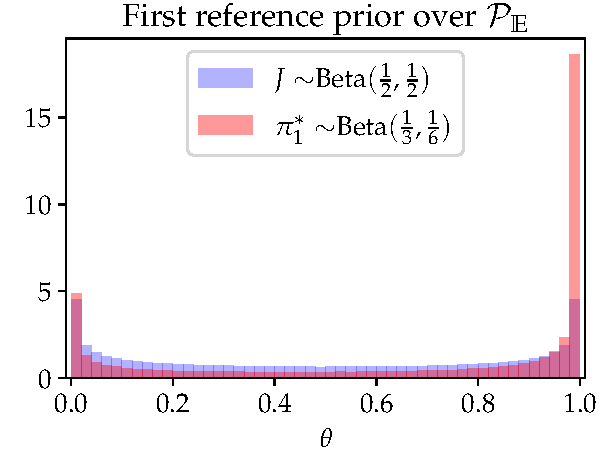
\includegraphics[width=5cm]{figures/generalized-ref/firstPe.pdf}\hspace*{0.5cm}%
    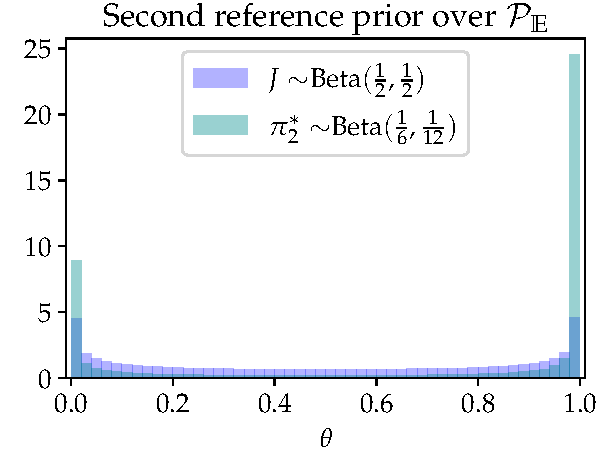
\includegraphics[width=5cm]{figures/generalized-ref/secondPe.pdf}\hspace*{0.5cm}%
    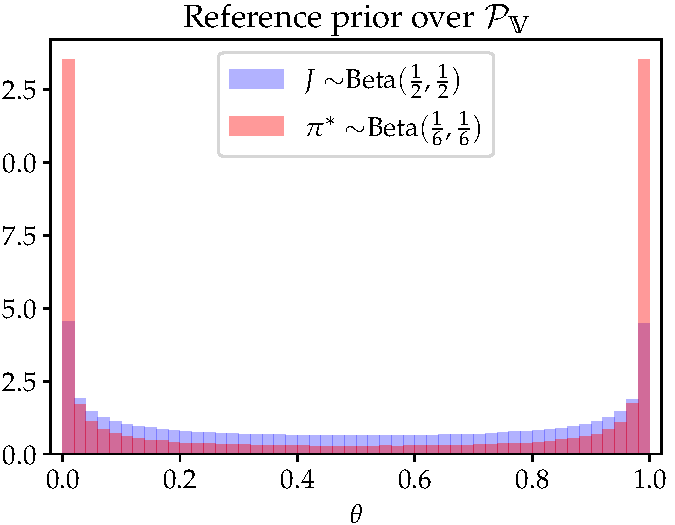
\includegraphics[width=5cm]{figures/generalized-ref/Pv.pdf}\\
    % \hspce*{0.16\linewidth}(a)
    \makebox[16cm][c]{%
    {\hspace{\stretch{1}}(a)\hspace{\stretch{2}}(b)\hspace{\stretch{2}}(c)\hspace{\stretch{1}}\ }%
    }
    % \begin{tabular}{ccc}
    %     (a) & (b)  & (c)
    % \end{tabular}
    \caption{Comparison of histograms of samples from Jeffreys prior and from the $D_f$-reference priors over a set $\cP_\EE=\{\pi=\mathrm{Beta},\,\EE_{T\sim\pi}T=\frac{2}{3}\}$ (\namecref{fig:exbeta} (a) and (b)), and over a set $\cP_\VV=\{\pi=\mathrm{Beta},\,\VV_{T\sim\pi}T=\frac{3}{16}\}$ (\namecref{fig:exbeta} (c)). In this example, their exist 2 solutions $\pi_1^\ast$ (in \namecref{fig:exbeta} (a)) and $\pi_2^\ast$ (in \namecref{fig:exbeta} (b)) of reference priors over $\cP_\EE$. $\delta$ has been set to $1/2$ in this example.}
    \label{fig:exbeta}
\end{figure}





    \subsection{About the assumptions and their limitations}

    The sub-Gaussian assumption over the likelihood, which is required for the statement of the result in the case $\delta<0$
    remains somehow restrictive. For instance,
    the univariate Gaussian model with unknown variance does not satisfy this assumption. 
    However, 
    it is still verified by other regular statistical models, such as the
    %it is still be verified by other regular statistical models, like the
     univariate normal model with known variance, or continuous compact models ($\cY$ compact and $(y,\theta)\mapsto\ell(y|\theta)$ continuously differentiable). {Note that due to the asymptotic normality of the r.v. $\cI(\theta)^{-1/2}S_k$ induced by the central limit theorem, the parameter $\xi$ of its assumed Gaussian tail cannot exceed $1/2$. This restricts $\delta$ to be smaller than $1$.}

Furthermore, %we would like to point out to the reader the two following remarks, raised from the proofs of our results.
in opposition with the classical settings for $f$-divergences which tend to suppose the convexity of $f$, the Jeffreys prior optimally within our results is actually implied by the concavity of $x\mapsto f(1/x)$ in the neighborhood of $0$.
This statement is showcased by the heuristic developed in the next subsection.

That gives some insight about the potential use of other functions $f$ than the ones we have considered.
Note that \citet{clarke_reference_1997} proved under some assumptions that another prior than Jeffreys prior is the $D$-reference prior when $D$ is a chi-square distance. This dissimilarity measure corresponds to the case where $f(x)=x^{-1}$, making $x\mapsto f(1/x)$ both convex and concave. 
A conclusion about the optimum of such generalized
mutual information thus requires stronger regularity assumptions on the likelihood to push
the asymptotic analysis further. %In their work, \citet{Clarke1997} have shown in a particular context that
%this could lead to the inverse of Jeffreys prior as the optimum.

%A global sketch of our proof giving an heuristic of the phenomena is proposed in Appendix~\ref{app:heuristic}. A rigorous proof is given in the next section.


    \subsection{About the robustness of Jeffreys prior with different divergences}


        \subsubsection{When $D_f$ is a $\delta=0$-divergence}

        The results elucidated in the previous section %a
        %re explicitly designed to 
        explicitly address $f$-divergences which are $\delta$-divergences.
        It is important to recall that when $\delta=0$, the $\delta$-divergence is usually defined as a  $\text{KL}$ divergence, more precisely it is an $f$-divergence with $f=-\log$.

        This way, the $\delta=0$-divergence leads to the original definition of the mutual information.
        In this case, 
        results similar to those of \cref{thm:PSGSA:Jrefdeltaneg,thm:PSGSA:Jrefdeltapos} exist (see \cref{chap:intro-ref}, \cref{sec:intro-ref:refpriors}). 
        



        \subsubsection{A heuristic for other $f$- divergences}

        We provide a heuristic for the derivation of the limit of a $D_f$-mutual information when $k\to\infty$. It is similar to discussions conducted by \citet{mure_objective_2018} and \citet{xie_minimax_1997}.

        The result of \cref{prop:PSGSA:cvptheta} takes the form of asymptotic connection between $p_{\mbf Y_k}(\mbf Y_k)/\ell_k(\mbf Y_k|\theta) $ and $e^{\frac{1}{2}S_k^T\cI(\theta)^{-1}S_k}$. This connection can be anticipated from the second order Taylor expansion written as follows: for every $\mbf y,\theta, \tilde\theta$, there exists a $\theta'$ in the segment between $\theta$ and $\tilde\theta$ such that
        \begin{equation}
            \log\left(\frac{\prod_{i=1}^k \ell(y_i|\tilde\theta)}{\prod_{i=1}^k \ell(y_i|\theta)}\right) = (\tilde\theta-\theta)^T\sum_{i=1}^k\nabla_\theta\log \ell(y_i|\theta) +\frac{1}{2}(\tilde\theta-\theta)^T\sum_{i=1}^k\nabla_\theta^2\log \ell(y_i|\theta')(\tilde\theta-\theta).
        \end{equation}
        Indeed, $p_{\mbf Y_k}(\mbf Y_k)/\ell_k(\mbf Y_k|\theta) = \int_\Theta \frac{\prod_{i=1}^k \ell(Y_i|\tilde\theta)}{\prod_{i=1}^k \ell(Y_i|\theta)} \pi(\tilde\theta)d\tilde\theta$.
        %When we exponentialize the Taylor expansion,
        % the first term 
        The terms $\nabla_\theta^2\log\ell_k(y_i|\theta)$ are definite negative, so that when we exponentialize the Taylor expansion, they vanish quickly when $\tilde\theta$ is not close to $\theta$.
        
        %We then intuit that the mass concentrate around 
        We deduce that the mass is concentrated around
        $\theta$ in the integrals that define $p_{\mbf Y_k}(\mbf Y_k)/\ell_k(\mbf Y_k|\theta)$, so that
            \begin{equation}
                \begin{aligned}
                p_{\mbf Y_k}(\mbf Y_k)/\ell_k(\mbf Y_k|\theta) &\approx \pi(\theta)\int_\Theta\exp\left(\sqrt{k}(\tilde\theta-\theta)^TS_k - \frac{k}{2} (\tilde\theta-\theta)^T\cI(\theta)(\tilde\theta-\theta)  \right)d\tilde\theta\\ 
                &= \pi(\theta)(2\pi)^{d/2}|k\cI(\theta)|^{-1/2}\exp\left(\frac{1}{2}S_k^T\cI(\theta)^{-1}S_k \right).
                \end{aligned}
            \end{equation} 

        % This approximation can be seen as a Berstein Von-Mises-like theorem, noticing that $p_{\mbf Y_k}(\mbf Y_k)/\ell_k(\mbf Y_k|\theta)$ equals $ \pi(\theta)/p(\theta|\mbf Y_k)$. 
        % , with the posterior 
        % being asymptotically a Gaussian with mean $\theta$ and variance $\cI(\theta)/\sqrt{k}$.
        %  asymtotically contionally to $T=\theta$ 

        To go toward an asymptotic expression of the mutual information, we must evaluate the last term with $f$ and compute its expectation w.r.t. $S_k$.
        Conditionally to $\theta$, the terms $\nabla_\theta\log\ell(Y_i|\theta)$ are i.i.d. and a central limit theorem gives that $(S_k)_k$ converges in distribution to a Gaussian with mean $\EE_{\theta}\nabla_\theta\log\ell(Y|\theta)=0$ and covariance matrix $\cI(\theta)$.
        
        That leads to approximating the $D_f$-mutual information  as 
            \begin{equation}\label{eq:PSGSA:heuristicconcave}
                \sI_{D_f}^k(\varPi) \approx \int_\Theta\int_{\RR^k} f\left(\pi(\theta)(2\pi)^{d/2}|k\cI(\theta)|^{-1/2}e^{\frac{\|x\|^2}{2}}\right) e^{-\frac{\|x\|^2}{2}} (2\pi)^{-d/2}dx\pi(\theta)d\theta.
            \end{equation}
        We notice that if $x\mapsto f(1/x)$ is concave, the right-hand term in the above equation is smaller than 
            \begin{equation}
                 \int_{\RR^k}f\left(\left(\int_\Theta (2\pi)^{-d/2}|k\cI(\theta)|^{1/2} e^{-\frac{\|x\|^2}{2}}d\theta\right)^{-1}\right)e^{-\frac{\|x\|^2}{2}}(2\pi)^{-d/2}dx ,
            \end{equation}
        which equals the right-hand term in \cref{eq:PSGSA:heuristicconcave} evaluated with $\pi(\theta) = |k\cI(\theta)|^{1/2} / \int_\Theta|k\cI(\tilde\theta)|^{1/2} d\tilde\theta$.

        This simple heuristic emphasizes that the decisive assumption on $f$ is that $x\mapsto f(1/x)$ is concave, rather than $f$ being convex.
        Regarding our developments in  \cref{sec:PSGSA:towardsdelta}, the final results on the optimally of Jeffreys stood while $a(\delta+1)>0$.
        In our cases, this condition implies the convexity of $f$ in the neighborhood of $0$, that is equivalent in these cases to $x\mapsto f(1/x)$ being concave in the neighborhood of $0$.
        



        
        \subsubsection{A simple development with a Maximum Mean Discrepancy divergence}


        We also investigate briefly the $D$-mutual information in a case where $D$ is not an $f$-divergence. The dissimilarity measure we have chosen to study is a squared maximum mean discrepancy (MMD):
                \begin{equation}
                    \text{MMD}^2(\cH;\,P||Q) = \EE_{X,X'\sim P\otimes P}[K(X,X')] + \EE_{Y,Y'\sim Q\otimes Q}[K(Y,Y')] - 2\EE_{X,Y\sim P\otimes Q}[K(X,Y)];
                \end{equation}
        where $\cH$ is a reproducing kernel Hilbert space (RKHS), and $K$ is a reproducing kernel.

        We study the simple Gaussian model with unknown mean: $\cY=\RR$, $\Theta\subset\RR $, and $\ell(y|\theta)=\frac{1}{\sqrt{2\pi}\sigma}e^{-\frac{(y-\theta)^2}{2\sigma^2}}$. 
        We consider the kernels $K_k:\mbf y,\mbf y'\in\cY^k,\,K_k(\mbf y,\mbf y')= \frac{1}{(\sqrt{2\pi}h)^k}e^{-\frac{\|\mbf y-\mbf y'\|^2}{2h^2}}$, and $\cH_k$ their associated RKHS. 
        For any $k$ it is thus possible to define the MMD between $\PP_{\mbf Y_k}$ and $\PP_{\mbf Y_k|\theta}$ by considering the RKHS $\cH_k$.
        Let $\tilde\Theta\subset\Theta$ be compact. %This way, for a prior
        For some prior $\varPi\in\sM^\nu_\cC$, denoting $\pi\in\sR_{\cC^b}$ a  density of $\varPi(\cdot|\tilde\Theta)$ we then have
            \begin{multline}
                \sI_{\text{MMD}^2}(\varPi(\cdot|\tilde\Theta)) =\frac{1}{(2\pi)^{3k/2} h^k\sigma^{2k}} \int_{\tilde\Theta}\int_{\RR^k\times\RR^k} \prod_{i=1}^ke^{-\frac{(y_i-y_i')^2}{2h^2}} e^{-\frac{(y_i-\theta)^2}{2\sigma^2} } e^{-\frac{(y_i'-\theta)^2}{2\sigma^2} }  d\mbf yd\mbf y'\pi(\theta)d\theta \\
                - \frac{1}{(2\pi)^{3k/2}h^k\sigma^{2k}} \int_{\tilde\Theta\times\tilde\Theta}\int_{\RR^k\times\RR^k} \prod_{i=1}^ke^{-\frac{(y_i-y_i')^2}{2h^2}} e^{-\frac{(y_i-\theta)^2}{2\sigma^2} } e^{-\frac{(y_i'-\theta')^2}{2\sigma^2} }  d\mbf yd\mbf y'\pi(\theta)\pi(\theta')d\theta d\theta'.
            \end{multline}

    In this very specific case, it is possible to derive and study the $\text{MMD}^2$-reference priors. The proposition below summarizes our results.
    
    \begin{prop}
        Let $\tilde\Theta\subset\Theta$ be a compact set. 
        \begin{enumerate}
            \item Let $\varPi,\,\tilde\varPi\in\sM^\nu_\cC$, we denote respectively $\pi$ and $\tilde\pi$ the densities of $\varPi(\cdot|\tilde\Theta)$ and $\tilde\varPi(\cdot|\tilde\Theta)$. We have:
            \begin{equation}
                \lim_{k\rightarrow\infty} C_1^{-k+1}\sqrt{k}(\sI_{\text{MMD}^2}(\varPi(\cdot|\tilde\Theta))-\sI_{\text{MMD}^2}(\tilde\varPi(\cdot|\tilde\Theta)) ) = -\int_{\tilde\Theta}\pi(\theta)^2d\theta + \int_{\tilde\Theta}\tilde\pi(\theta)^2d\theta,
            \end{equation}
            with $C_1=\frac{(2\sigma^2+h^2)^{-1/2}}{\sqrt{2\pi}}$.
            %If not jeffreys then $>0$.
            And the Jeffreys prior class is the unique $\text{MMD}^2$-reference prior class over $\sM^\nu_\cC$.
            \item For a density $\pi$ %such that $\int_{\tilde\Theta}\pi =1$ 
            we denote by $M(\pi)$ its associated normalized prior: $M(\pi)=B\mapsto\int_B\pi/\int_{\tilde\Theta}\pi$.
            %Denote $\cC(\tilde\Theta)$
            Let $\pi^\ast_k$ be continuous densities such that for any $k$, $\sI_{\text{MMD}^2}(M(\pi^\ast_k))\geq \sI^k_{\text{MMD}^2}(M(\pi))$ for any other  $\pi\in\sM^\nu_\cC$.
            If $(\pi^\ast_k)_k$ converges uniformly to a function $\pi^\ast$ on $\tilde\Theta$, then $\pi^\ast$ is the Jeffreys prior density: $\pi^\ast\propto1$.
        \end{enumerate}
    \end{prop}

\begin{proof}
    First we derive for any $\theta,\theta'\in\tilde\Theta$
            \begin{multline}
                \int_{\RR\times\RR} e^{-\frac{(y-y')^2}{2h^2}} e^{-\frac{(y-\theta)^2}{2\sigma^2} } e^{-\frac{(y'-\theta')^2}{2\sigma^2} }  d yd y' 
                    \\
                    \begin{aligned}
                        &= \sqrt{2\pi\tilde\sigma^2}\int_{\RR} e^{-\frac{y'^2}{2h^2}}e^{-\frac{\theta^2}{2\sigma^2}} e^{\frac{1}{2\tilde\sigma^2}\left( \frac{\tilde\sigma^2}{h^2}y'+\frac{\tilde\sigma^2}{\sigma^2}\theta \right)^2} e^{-\frac{(y'-\theta')^2}{2\sigma^2}}dy'
                        &\mbox{with }\tilde\sigma^{-2}=\frac{1}{h^2}+\frac{1}{\sigma^2}\\
                    & = 2\pi\tilde\sigma\overline\sigma
                    e^{-\frac{\theta^2}{2\sigma^2}} e^{-\frac{\theta'^2}{2\sigma^2}} e^{\frac{1}{2}\frac{\tilde\sigma^2}{\sigma^4}\theta^2} e^{\frac{1}{2\overline\sigma^2}\left(\frac{\overline\sigma^2}{\sigma^2}\theta' - \frac{\overline\sigma^2\tilde\sigma^2}{h^2\sigma^2}\theta\right)^2} 
                        &\mbox{with }\overline\sigma^{-2}= \frac{1}{h^2} - \frac{\tilde\sigma^2}{h^4} + \frac{1}{\sigma^2} = \frac{1}{\sigma^2+h^2}+\frac{1}{\sigma^2}\\
                    &= 2\pi\tilde\sigma\overline\sigma e^{-\frac{1}{2}\frac{1}{2\sigma^2+h^2}\left(\theta' - \theta\right)^2}. 
                    \end{aligned}
            \end{multline}
        That allows us to write
    \begin{equation}\label{eq:PSGSA:expr2IMMD}
        \sI_{\text{MMD}^2}(\varPi(\cdot|\tilde\Theta)) = - C_1^k\int_{\tilde\Theta\times\tilde\Theta} e^{-\frac{k}{2}\frac{1}{2\sigma^2+h^2}(\theta'-\theta)^2}\pi(\theta)\pi(\theta')d\theta d\theta' + C_1^k,
    \end{equation}
with $C_1=\frac{\tilde\sigma\overline{\sigma}}{\sqrt{2\pi}h\sigma^2} = \frac{(2\sigma^2+h^2)^{-1/2}}{\sqrt{2\pi}}$. %From the above expression, it is possible to develop two approaches to construct a reference prior in this very specific case:
%\begin{itemize}
 %   \item 
 \begin{enumerate}
    \item To prove the first statement of the theorem, 
    we start by  computing the limit as $k\to\infty$ of the integrals  $C_1\sqrt{k}\int_{\tilde\Theta}e^{-\frac{k}{2}\frac{1}{2\sigma^2+h^2}(\theta'-\theta)^2}\pi(\theta)d\theta $ for a fixed $\theta'$ in which $\pi$ is continuous. The scheme of this proof is standard as this integral is the convolution of  $\pi$ with an approximate Dirac distribution. %to the unity. 
    Let $\eps>0$, by continuity of $\pi$ there exists a neighborhood $V$ of $\theta'$ such that for any $\theta\in V$,  $|\pi(\theta)-\pi(\theta')|<\eps/2$. %for any $\theta\in V$.
    Additionally, it is possible to choose a $k_0$ such that for all $k\geq k_0$, $C_1\sqrt{k}\int_{\RR\!\setminus\!V} e^{-\frac{k}{2}\frac{(\theta'-\theta)^2}{2\sigma^2+h^2}}d\theta <\eps/(4\sup_{\tilde\Theta}\pi)$. This way, for all $k\geq k_0$,
        \begin{equation}
            \left|C_1\sqrt{k}\int_{\tilde\Theta}e^{-\frac{k}{2}\frac{1}{2\sigma^2+h^2}(\theta'-\theta)^2}\pi(\theta)d\theta -\pi(\theta')  \right| \leq C_1\sqrt{k}\int_{\RR}e^{-\frac{k}{2}\frac{1}{2\sigma^2+h^2}(\theta'-\theta)^2} |\pi(\theta)\indic_{\theta\in\tilde\Theta}-\pi(\theta')|d\theta 
            <\eps.
        \end{equation}
    
    That being stated, we can apply a dominated convergence theorem since for $\nu$-a.e. $\theta'$ and for all $k$, the terms $|C_1\sqrt{k}\int_{\tilde\Theta} e^{-\frac{k}{2}\frac{(\theta-\theta')^2}{2\sigma^2+h^2}}\pi(\theta)\pi(\theta')d\theta |\leq(\sup_{\tilde\Theta}\pi)^2$, which is summable on $\tilde\Theta$.
    We obtain
    \begin{equation}
        \lim_{k\rightarrow\infty} C_1^{-k+1}\sqrt{k}(\sI_{\text{MMD}^2}(\varPi(\cdot|\tilde\Theta))-\sI_{\text{MMD}^2}(\tilde\varPi(\cdot|\tilde\Theta)) ) = -\int_{\tilde\Theta}\pi(\theta)^2d\theta + \int_{\tilde\Theta}\tilde\pi(\theta)^2d\theta.
    \end{equation}
    We recall that the Jeffreys prior $\mbf J $ for this model is the uniform prior: $J\propto 1$.
    Since Chauchy-Schwarz inequality implies $\int_{\tilde\Theta}\tilde\pi(\theta)d\theta \leq \sqrt{\nu(\tilde\Theta)} \left(\int_{\tilde\Theta}\pi(\theta)^2d\theta \right)^{1/2}$, with equality if and only if $\tilde\pi\propto 1$, we deduce 
    \begin{equation}
        \lim_{k\rightarrow\infty} C_1^{-k+1}\sqrt{k}(\sI_{\text{MMD}^2}(\mbf J(\cdot|\tilde\Theta))-\sI_{\text{MMD}^2}(\tilde\varPi(\cdot|\tilde\Theta)) ) \geq 0 \text{\ with equality iff\ }\mbf J(\cdot|\tilde\Theta) = \tilde\varPi(\cdot|\tilde\Theta).
    \end{equation}

\item We consider the vectorial space $\cC(\tilde\Theta)$ of continuous real functions defined on $\tilde\Theta$. It is a Banach space when equipped with the norm $\|p\|=\sup_{\tilde\Theta}|p|$. The expression of $\sI_{\text{MMD}^2}(\varPi(\cdot|\tilde\Theta))$ elucidated in \cref{eq:PSGSA:expr2IMMD} can be seen as a functional of $\pi$ of the form $\pi\mapsto B(\pi,\pi)$, $B$ being a continuous bilinear form on $E^2$. This function is differentiable w.r.t. $\pi$. We thus  apply a Lagrange multipliers theorem to write that if $\pi_k^\ast\in E$ maximizes $\pi\mapsto\sI^k_{\text{MMD}^2}(\varPi(\cdot|\tilde\Theta))$ on the constrained space $E\cap\{p\in E,\,\int_{\tilde\Theta}p=1\}$, then there exists $\lambda\in\RR$ such that for all $p\in E$:
\begin{equation}
    -2C_1^k\int_{\Theta\times\Theta} e^{-\frac{k}{2}\frac{1}{2\sigma^2+h^2}(\theta-\theta')^2} p(\theta)\pi^\ast_k(\theta')d\theta d\theta' - \lambda\int_\Theta p(\theta)d\theta = 0.
\end{equation}
This being true for any $p\in E$, we deduce for all $\theta'\in\tilde\Theta$, %setting $p(\theta) = C_1\sqrt{k} $
    \begin{equation}
        -2C_1^k\int_{\tilde\Theta} e^{-\frac{k}{2}\frac{(\theta'-\theta)^2}{2\sigma^2+h^2}} \pi_k^\ast(\theta)d\theta = \lambda \quad\text{and}\quad
        -2C_1^k\int_{\tilde\Theta\times\tilde\Theta} e^{-\frac{k}{2}\frac{(\theta'-\theta)^2}{2\sigma^2+h^2}} \pi_k^\ast(\theta)\pi_k^\ast(\theta')d\theta d\theta' = \lambda.
    \end{equation}
We now apply a similar reasoning as in 1. to derive the limits of the above integrals. 
The $\pi^\ast_k$ are assumed to form a uniformly convergent sequence of functions. That ensures its limit $\pi^\ast$ is continuous on $\tilde\Theta$.
We fix $\theta'\in\tilde\Theta$. Let $\eps>0$, we fix a neighborhood $V$ of $\theta'$ such that for all $\theta \in V$, $|\pi^\ast(\theta)-\pi^\ast(\theta')|<\eps/4$. By uniform convergence of $(\pi^\ast_k)$, we can fix $k_0$ such that for all $k\geq k_0$, $\|\pi^\ast_k-\pi^\ast\|<\eps/4$. It is also possible to fix $k_1$ such that for all $k\geq k_1$, $C_1\sqrt{k}\int_{\RR\!\setminus\!V} e^{-\frac{k}{2}\frac{(\theta'-\theta)^2}{2\sigma^2+h^2}}d\theta <\eps/(8\sup_{k'}\|\pi^\ast_{k'}\|)$.
    We thus have for all $k\geq\max(k_1,k_0)$
    \begin{equation}
        \begin{aligned}
        &\left|C_1\sqrt{k}\int_{\tilde\Theta } e^{-\frac{k}{2}\frac{(\theta'-\theta)^2}{2\sigma^2+h^2}} \pi^\ast_k(\theta)d\theta - \pi^\ast(\theta') \right| 
        \leq C_1\sqrt{k}\int_{\RR}e^{-\frac{k}{2}\frac{(\theta'-\theta)^2}{2\sigma^2+h^2}} |\pi^\ast_k(\theta)\indic_{\theta\in\Theta} - \pi^\ast(\theta') |d\theta \\
        &\leq  C_1\sqrt{k}\int_{\RR}e^{-\frac{k}{2}\frac{(\theta'-\theta)^2}{2\sigma^2+h^2}} |\pi^\ast_k(\theta)\indic_{\theta\in\Theta} - \pi^\ast(\theta)\indic_{\theta\in\Theta} |d\theta 
            + C_1\sqrt{k}\int_{\RR}e^{-\frac{k}{2}\frac{(\theta'-\theta)^2}{2\sigma^2+h^2}} |\pi^\ast(\theta)\indic_{\theta\in\Theta} - \pi^\ast(\theta') |d\theta <\eps.\\
        %&+ C_1\sqrt{k}\int_{\RR}e^{-\frac{k}{2}\frac{(\theta'-\theta)^2}{2\sigma^2+h^2}} |f(\theta)\indic_{\theta\in\Theta} - f(\theta') |d\theta  < 
        \end{aligned}
        \end{equation}
        As the integrated terms are all bounded, a dominated converge theorem gives:
        \begin{equation}
            \begin{aligned}
            &\lim_{k\rightarrow\infty}C_1\sqrt{k}\int_{\tilde\Theta} e^{-\frac{k}{2}\frac{(\theta'-\theta)^2}{2\sigma^2+h^2}} \pi_k^\ast(\theta)d\theta = \pi^\ast(\theta')\\
            \text{and}\quad&
            \lim_{k\rightarrow\infty} C_1\sqrt{k}\int_{\tilde\Theta\times\tilde\Theta} e^{-\frac{k}{2}\frac{(\theta'-\theta)^2}{2\sigma^2+h^2}} \pi_k^\ast(\theta)\pi_k^\ast(\theta')d\theta d\theta' = \int_{\tilde\Theta}\pi^\ast(\theta)^2d\theta.
            \end{aligned}
        \end{equation}
        Since the above terms are equal, we conclude that $\pi^\ast$ is constant.





 \end{enumerate}
\end{proof}


\section{Proofs of the main results}\label{sec:PSGSA:proofs}

\subsection{Proof of the convergence in probability}

\begin{proofb}[Proof of \cref{prop:PSGSA:cvptheta}]
    We fix $\theta$ in the interior of $\Supp\pi$ such that $\pi$ is continuous in $\theta$. Let $\eps,\tilde\eps>0$. We want to show that there exist $k_0$, such that for all $k\geq k_0$
        \begin{equation}
            \PP_\theta\left(\tilde g_2^{C,c}(k^{-d/2})^{-1}\left| f\left(\frac{p_{\mbf Y_k}(\mbf Y_k)}{\ell_k(\mbf Y_k|\theta)}\right) \right.            \left. - g_1\left(k^{-d/2}\pi(\theta)(2\pi)^{d/2}|\cI(\theta)|^{-1/2}\exp\left(\frac{1}{2}S_k^T\cI(\theta)^{-1}S_k \right)\right) \right|<\tilde\eps   \right)>1-\eps,
        \end{equation}
    for some $C,c = C_\theta,c_\theta$.
    We start by defining some events that 
    will be asymptotically negligible:
    \begin{enumerate}
    \item Remind the definition of the r.v. $S_k=\frac{1}{\sqrt{k}}\sum_{i=1}^k\nabla_\theta\log\ell(Y_i|\theta)$. The central limit theorem ensures that when $\mbf Y_k\sim\PP_{\mbf Y_k|\theta}$, $S_k$ converges in distribution to $\cN(0,\cI(\theta))$ as $k\to\infty$. Therefore, one can choose $M_\theta$ such that the events $ \underline{\mbf A}_k(\theta)$ defined as $ \underline{\mbf A}_k(\theta)=\{\|S_k\|>M_\theta\}$ verify
        \begin{equation}
            \PP_\theta( \underline{\mbf A}_k(\theta))\conv{k\rightarrow\infty}\eps/5
        \end{equation}
    
        \item Denote for any $i=1,\dots,k$, and for any $\mbf y \in\cY^k$,
        \begin{equation}
            \kappa_i(\mbf y)=\{-x^T\nabla^2_\theta\log\ell(y_i|\theta')x,\,\theta'\in\tilde\Theta,\,\|x\|=1\}.
        \end{equation}
     They are compact subsets of $(0,+\infty)$. The law of large numbers gives 
     \begin{equation}
        \frac{1}{k}\sum_{i=1}^k\inf \kappa_i(\mbf Y_k)\conv{k\rightarrow\infty}\EE_\theta\left[\inf_{\theta'\in\tilde\Theta,\|x\|=1}-x^T\nabla^2_\theta\log\ell(Y_1|\theta')x\right]  ,
     \end{equation}
    which is positive as the infima are positive $\PP_\theta$-a.s. We choose an $\hat m_\theta>0$ smaller than this limit, and we denote
        \begin{equation}
             \underline{\mbf B}_k(\theta)=\left\{\frac{1}{k}\sum_{i=1}^k\inf \kappa_i(\mbf Y_k)<\hat m\right\}.       
        \end{equation}
     Then $\PP_\theta( \underline{\mbf B}_k(\theta))\conv{k\rightarrow\infty}0$.

    \item Beforehand, denote
    \begin{equation}
        C_\theta =\exp\left(M_\theta^2/(2\hat m_\theta)\right) \quad\text{and}\quad  c_\theta = \pi(\theta)(2\pi)^{d/2}|\cI(\theta)|^{-1/2} ,
    \end{equation}
    which are finite and positive. Using the assumed local behavior of $f$ around $0$, one can choose $ w,\eta>0$ such that for any $c_\theta<|x|<C_\theta$, $|l|< w$, and $|t|<\eta$, 
    \begin{equation}\label{eq:PSGSA:asymptdevf}
        |f(xt+lt)-g_1(xt)|\leq\tilde\eps g_2(xt)\leq\tilde\eps\tilde g_2^{C_\theta,c_\theta}(t).    
    \end{equation}
    Using the $\PP_\theta$-a.s. convergence of $-\frac{1}{k}\sum_{i=1}^k\nabla^2_\theta\log\ell(Y_i|\theta)$ to $\cI(\theta)$, we have $\PP_\theta( \underline{\mbf C}_k(\theta))\conv{k\rightarrow\infty}0$ where
    \begin{align}
    \nonumber
         \underline{\mbf C}_k(\theta) = &\left\{\forall \|x\|\leq M,\, \left|\pi(\theta)(2\pi)^{d/2}|k\cI(\theta)|^{-1/2}\exp\left(\frac{1}{2}x^T \cI(\theta)^{-1}x\right) \right.\right. \\
        & \left.\left. - \pi(\theta)(2\pi)^{d/2}|k\hat\cI_k(\theta)|^{-1/2}\exp\left(\frac{1}{2}x^T \hat\cI_k(\theta)^{-1} x\right) \right|\geq w k^{-d/2}\right\} ,
    \end{align}
    with $\hat\cI_k(\theta')$ denoting $-\frac{1}{k}\sum_{i=1}^k\nabla^2_\theta\log\ell(Y_i|\theta')$.
    
    \item 
    Let us choose $R_\theta>0$ large enough to have 
    \begin{equation}\label{eq:PSGSA:majorintegralsR}
        (\sup_{\tilde\Theta}\pi ) \int_{\|x\|>R_\theta} e^{M_\theta x}e^{-\frac{\hat m_\theta}{2}x^2} dx< w ,    
    \end{equation}
and $u>0$ such that $\forall|x|<uR_\theta^2,\,|e^{x}-1|< w/(2 C_\theta R^d_\theta\sup_{\tilde\Theta}\pi )$. 

From \cref{assu:intro-ref:jeffreysexist}, the function $\theta'\mapsto\|\nabla_\theta^2\log\ell(y|\theta')-\nabla^2_\theta\log\ell(y|\theta)\|$ is dominated on the Euclidean ball $B(\theta,\tau_1)$ by a variable that has a finite expectation $\EE_\theta$. Therefore, a dominated convergence theorem gives that the function
    \begin{equation}
        \theta'\mapsto \EE_\theta \left[\|\nabla_\theta^2\log\ell(Y_1|\theta')-\nabla^2_\theta\log\ell(Y_1|\theta)\|\right]
    \end{equation}
    converges to $0$ when $\theta'\to\theta$ as a consequence of the continuity of the second order partial derivatives of the log-likelihood. 
    
    
    Thus, {if we choose $\tilde\tau_\theta$ such that the above quantity is smaller than %$\eps\nu\sup_{\tilde\Theta}\pi/(10\cdot D^d)$ 
    $u\eps$ and if we define $\underline{\mbf D}_k(\theta)$ as the event}
    \begin{equation}
        \underline{\mbf D}_k(\theta)=\left\{\sup_{\theta'\in\tilde\Theta,\,\|\theta'-\theta\|<\tilde\tau_\theta}\|\hat\cI_k(\theta')-\hat\cI_k(\theta)\|>u \right\}, %\nu\sup_{\tilde\Theta}\pi/(2D^d) \right\},
    \end{equation}
    one gets by applying Markov's inequality that $\PP_\theta(\underline{\mbf D}_k(\theta))<\eps/4$.
    \end{enumerate}

    Now, notice that for any $\tilde\theta\in\tilde\Theta$, $\mbf y\in\cY^k$, there exists $\hat\theta$ on the segment between $\theta$ and $\tilde\theta$ such that
    \begin{equation}\label{eq:DLlogfraclik}
        \log\left(\frac{\prod_{i=1}^k \ell(y_i|\tilde\theta)}{\prod_{i=1}^k \ell(y_i|\theta)}\right) = (\tilde\theta-\theta)^T\sum_{i=1}^k\nabla_\theta\log \ell(y_i|\theta) +\frac{1}{2}(\tilde\theta-\theta)^T\sum_{i=1}^k\nabla_\theta^2\log \ell(y_i|\hat\theta)(\tilde\theta-\theta).
    \end{equation}
    Let us write %$D_f(\PP_{\mbf Y}||\PP_{\mbf Y|T=\theta})=\EE_\theta\left[f\left(\int_\Theta h_{ \mbf y}(\tilde\theta,\theta)\pi(\tilde\theta)d\tilde\theta\right)\right]$ where
    $p_{\mbf Y_k}(\mbf y)/\ell_k(\mbf y|\theta) = \int_\Theta h_{\mbf y}(\tilde\theta,\theta)\pi(\tilde\theta)d\tilde\theta$ where
    \begin{equation}\label{eq:hydef}
        h_{\mbf y}(\tilde\theta,\theta) = \exp\left((\tilde\theta-\theta)^T\nabla_\theta\log\ell_k(\mbf y|\theta)\right)  \exp \left( \frac{1}{2}(\tilde\theta-\theta)^T\nabla^2_\theta\log\ell_k(\mbf y|\hat\theta)(\tilde\theta-\theta) \right).
    \end{equation}
    We fix $k$ and work under the event $\underline{\mbf A}_k(\theta)^c\cap \underline{\mbf B}_k(\theta)^c\cap \underline{\mbf C}_k(\theta)^c\cap \underline{\mbf D}_k(\theta)^c$. i.e. we %fix $\mbf y\in\cY^k$ such that 
    consider $\varpi\in \underline{\mbf A}_k(\theta)^c\cap \underline{\mbf B}_k(\theta)^c\cap \underline{\mbf C}_k(\theta)^c\cap \underline{\mbf D}_k(\theta)^c$ and denote $\mbf y = \mbf Y_k(\varpi)$, $ S_k^{\mbf y}=\frac{1}{\sqrt{k}}\nabla_\theta\log\ell_k(\mbf y|\theta)$, $\hat\cI_k^{\mbf y}(\theta) =-\frac{1}{k}\nabla^2_\theta\log\ell_k(\mbf y|\theta) $.
    We can thus bound $h_{\mbf y}(\tilde\theta,\theta)$  as
    \begin{equation}\label{eq:inegh}
        h_{\mbf y}(\tilde\theta,\theta) \leq\exp\left( M_\theta\sqrt{k}\|\tilde\theta-\theta\| \right)\exp\left( -\frac{k}{2}\hat m_\theta\|\tilde\theta-\theta\|^2 \right)\leq C_\theta.
    \end{equation}
    
    The rest of the proof only consists in bounding  four  quantities by $ w k^{-d/2} $.
    \begin{itemize}
        \item Define $\tilde R_k=R_\theta k^{-1/2}$. %with a $D>0$ thin enough to have $\int_{\|x\|>D}e^{Mx}e^{-\frac{m}{2}x^2}\sup_{\tilde\Theta}|\pi|dx<\nu$ and to let the Euclidean ball $B(\theta,D)\subset\tilde\Theta$.
        Inequality in \cref{eq:PSGSA:majorintegralsR} implies
        \begin{equation}
            \mbf I_1 := \int_{\|\tilde\theta-\theta\|>\tilde R_k} \exp\left((\tilde\theta-\theta)^T\sqrt{k}S_k^{\mbf y}\right)\exp\left( -\frac{k}{2}(\tilde\theta-\theta)^T\hat\cI_k^{\mbf y}(\theta)(\tilde\theta-\theta) \right)\pi(\theta)d\tilde\theta < w k^{-d/2}.
        \end{equation}
        \item Recalling the upper bound in \cref{eq:inegh}, we have the same way
            \begin{equation}
                \mbf I_2 := \int_{\|\tilde\theta-\theta\|>\tilde R_k} h_{\mbf y}(\tilde\theta,\theta)\pi(\tilde\theta)d\tilde\theta < w k^{-d/2}.
            \end{equation}
        \item  
        As $\pi$ is continuous in $\theta$, 
        there exist $k_1$ such that if $k\geq k_1$ then for all $\|\tilde\theta-\theta\|<\tilde R_k$, $|\pi(\tilde\theta)-\pi(\theta)|\leq w/(2C_\theta R_\theta^d)$. %for any $\|\tilde\theta-\theta\|<\tilde R_k$. 
        We write:
            \begin{multline}\label{eq:continuityofHatIk}
               \mbf I_3 := \int_{\|\tilde\theta-\theta\|<\tilde R_k} h_{\mbf y}(\tilde\theta,\theta)\pi(\tilde\theta)d\tilde\theta  
                     - \int_{\|\tilde\theta-\theta\|<\tilde R_k}\exp\left((\tilde\theta-\theta)^T\sqrt{k}S_k^{\mbf y}\right)\exp\left(-\frac{k}{2}(\tilde\theta-\theta)^T\hat\cI_k^{\mbf y}(\theta)(\tilde\theta-\theta)\right)\pi(\theta)d\tilde\theta \\ %\leq\nu k^{-d/2}.
                %
                    |\mbf I_3| \leq \int_{\|\tilde\theta-\theta\|<\tilde R_k}|\hat h_{\mbf y}(\tilde\theta,\theta,\hat\theta) - \hat h_{\mbf y}(\tilde\theta,\theta,\theta) |\pi(\tilde\theta)d\tilde\theta + \int_{\|\tilde\theta-\theta\|<\tilde R_k}\hat h_{\mbf y}(\tilde\theta,\theta,\theta)|\pi(\tilde\theta)-\pi(\theta)|d\tilde\theta
              %
            \end{multline}
        where $\hat h_{\mbf y}(\tilde\theta,\theta,\hat\theta)=\exp((\tilde\theta-\theta)^T\sqrt{k}S_k^{\mbf y})\exp\left(-\frac{k}{2}(\tilde\theta-\theta)^T\hat\cI_k^{\mbf y}(\hat\theta)(\tilde\theta-\theta)\right)$. {Notice that for any $\theta',\tilde\theta$ in the Euclidean ball $B(\theta,\tilde R_k)$,}
            \begin{align}   
                 |\hat h_{\mbf y}(\tilde\theta,\theta,\theta') - \hat h_{\mbf y}(\tilde\theta,\theta,\theta) | 
                    \leq \hat h_{\mbf y}(\tilde\theta,\theta,\theta')\left|\exp\left( -\frac{k}{2}(\tilde\theta-\theta)^T(\hat\cI_k^{\mbf y}(\theta')-\hat\cI_k^{\mbf y}(\theta))(\tilde\theta-\theta) \right)-1\right|.
            \end{align}
        Thus, if $k\geq k_2$ where $k_2$ is such that $\tilde R_{k_2}<\tilde\tau$, we obtain $(\tilde\theta-\theta)^T(\hat\cI_k^{\mbf y}(\theta')-\hat\cI_k^{\mbf y}(\theta))(\tilde\theta-\theta) < u$ consequently to $\mbf y=\mbf Y_k(\varpi)$ with $\varpi\in\underline{\mbf D}_k(\theta)^c$. 
        It then comes $|\mbf I_3|< w k^{-d/2}$.

        \item  By recognizing a Gaussian density in the integral below, we get the equality 
        \begin{align}
        \nonumber
            &\int_{\RR^d}\exp((\tilde\theta-\theta)^T\sqrt{k}S_k^{\mbf y})\exp\left(\frac{1}{2}(\tilde\theta-\theta)^T\nabla_\theta^2\ell_k(\mbf y|\theta)(\tilde\theta-\theta)\right)\pi(\theta)d\tilde\theta \\
            &=
            \pi(\theta)(2\pi)^{d/2}|k\hat\cI_k^{\mbf y}(\theta)|^{-1/2}\exp\left(\frac{1}{2}S_k^{\mbf y T}\hat\cI_k^{\mbf y}(\theta)^{-1}S_k^{\mbf y}\right).
            \label{eq:intRnabla2bisbis}
        \end{align}
        Defining $\mbf I_4= (\ref{eq:intRnabla2bisbis}) - \pi(\theta)(2\pi)^{d/2}|k\cI(\theta)|^{-1/2}\exp\left(\frac{1}{2}S_k^{\mbf yT}\cI(\theta)^{-1}S_k^{\mbf y}\right)$, we obtain,
        %It implies, 
        using that $\varpi\in \underline{\mbf C}_k(\theta)^c$, 
        \begin{equation}
            |\mbf I_4|  %\left|(\ref{eq:intRnabla2bisbis}) - \pi(\theta)(2\pi)^{d/2}|k\cI(\theta)|^{-1/2}\exp\left(\frac{1}{2}S_k^T\cI(\theta)^{-1}S_k\right)\right|
            \leq w k^{-d/2}.
        \end{equation}
    \end{itemize}

If we define $k_3$ such that $k^{-d/2}<\eta/4$, and if $k\geq\max(k_1,k_2,k_3)$, then the four inequalities elucidated above allows evaluating \cref{eq:PSGSA:asymptdevf} with $t=k^{-d/2}$,
\begin{equation}
    \begin{aligned}
    x(\mbf y) = & \int_{\tilde\Theta} \exp\left((\tilde\theta-\theta)^T\sqrt{k}S_k^{\mbf y}\right)\exp\left( -\frac{k}{2}(\tilde\theta-\theta)^T\hat\cI_k^{\mbf y}(\theta)(\tilde\theta-\theta) \right)\pi(\theta )d\tilde\theta,\\
        \text{and}\quad l(\mbf y) =&\, x(\mbf y)-\frac{p_{\mbf y}(\mbf y)}{\ell_k(\mbf y|\theta)}k^{d/2} = \mbf I_1+\mbf I_2+\mbf I_3+\mbf I_4.
    \end{aligned}
\end{equation}

All in all, we have proven that for $k\geq\max(k_1,k_2,k_3)$ the inclusion
    \begin{equation}
         \underline{\mbf A}_k(\theta)^c\cap \underline{\mbf B}_k(\theta)^c\cap \underline{\mbf C}_k(\theta)^c\cap \underline{\mbf D}_k(\theta)^c \subset \left\{ \left|f\left(\frac{p_{\mbf Y_k}(\mbf Y_k)}{\ell_k(\mbf Y_k|\theta)} \right) - g_1(k^{-d/2} x(\mbf Y_k)) \right| < \tilde g_2^{C_\theta,c_\theta}(k^{-d/2}) \tilde\eps  \right\}
    \end{equation}
stands.
To conclude we denote $k_4$ such that for any $k\geq k_4$,
        \begin{equation}
            \PP_\theta(\underline{\mbf A}_k(\theta)) <\eps/4,\quad\PP_\theta(\underline{\mbf B}_k(\theta))<\eps/4, \quad\PP_\theta(\underline{\mbf C}_k(\theta))\eps/4, \quad \PP_\theta(\underline{\mbf D}_k(\theta))<\eps/4.
        \end{equation}
This way, defining $k_0=\max(k_1,k_2,k_3,k_4)$, the following inequality is true for any $k\geq k_0$:
\begin{equation}
    \PP_\theta\left(\tilde g_2^{C_\theta,c_\theta}(k^{-d/2})^{-1}\left| f\left(\frac{p_{\mbf Y_k}(\mbf Y_k)}{\ell_k(\mbf Y_k|\theta)}\right) \right.            \left. - g_1\left(k^{-d/2}\pi(\theta)(2\pi)^{d/2}|\cI(\theta)|^{-1/2}\exp\left(\frac{1}{2}S_k^T\cI(\theta)^{-1}S_k \right)\right) \right|<\tilde\eps   \right)>1-\eps.
\end{equation}
\end{proofb}


\newcommand{\ubf}[1]{\underline{\mbf{#1}}}


\subsection{Proof of the results when $\delta<0$} %\cref{thm:refcompactneg,thm:PSGSA:Jrefdeltaneg}}

\begin{proofb}[Proof of \cref{thm:refcompactneg,prop:JlimIMdeltaneg,thm:PSGSA:Jrefdeltaneg}]
    We suppose that \cref{assu:PSGSA:JDS} is verified. We recall that in this proof $\delta<0$. The following lemma is required for the proof. It is proven later on.
    \begin{lem}
        \label{lem:dfbeta}
            Let $\zeta<0$. 
            There exists a constant $K$ independent of $\theta$ such that
                \begin{equation}
                    k^{d\zeta/2}\EE_\theta \left[\left(\frac{p_{\mbf Y_k}(\mbf Y_k)}{\ell_k(\mbf Y_k|\theta)}\right)^\zeta \right]\leq  K.
                \end{equation}
        \end{lem}

        We recall that \cref{prop:PSGSA:cvptheta} states the following convergence in probability for a.e. $\theta$:
\begin{equation}
    k^{d\delta/2}\left|f\left(\frac{p_{\mbf Y_k}(\mbf Y_k)}{\ell_k(\mbf Y_k|\theta)}\right)  - a k^{-d\delta/2}\pi(\theta)^\delta(2\pi)^{d\delta/2}|\cI(\theta)|^{-\delta/2}\exp\left(\frac{\delta}{2} S_k^T\cI(\theta)^{-1}S_k \right)  \right|
        \conv[\PP_\theta]{k\rightarrow\infty}0.
\end{equation}

The first goal in this prove will be to show that this convergence  is a convergence in $L^1(\PP_\theta)$. This is shown by proving that the sequence of r.v. is uniformly integrable. 
Let $\rho>0$ and choose an even $\ubf A$ such that $\PP_\theta(\ubf A)=\rho$. %Denoting $X_k=\cI(\theta)^{-1/2}S_k$,
Firstly, we have 
    \begin{equation}
        \EE_\theta\left[\indic_{\ubf A} \pi(\theta)^\delta(2\pi)^{d\delta/2}e^{\frac{\delta}{2}S_k^T\cI(\theta)^{-1}S_k}\right]  
        \leq \pi(\theta)^\delta(2\pi)^{d\delta/2} \rho,
    \end{equation}
and secondly,
considering  $t$,  $\hat C$ and $\hat C'$ such that $|f(x)|\leq\hat Cx$ if $x>t$ and $|f(x)|\leq \hat C'x^\delta$ otherwise; we obtain using 
$\ubf G_k= \ubf G_k(\theta)\{p_{\mbf Y}(\mbf y)>\gamma\ell_k(\mbf y|\theta)\}$ and Hölder's inequality:
    \begin{align}
%\nonumber      
 \EE_\theta\left[ \indic_{\ubf A}k^{d\delta/2}f\left( \frac{p_{\mbf Y_k}(\mbf Y_k)}{\ell_k(\mbf Y_k|\theta)}\right) \right]
%    
\nonumber                  
    &\leq \EE_\theta\left[ \indic_{\ubf G_k}\indic_{\ubf A} k^{d\delta/2} \hat C  \frac{p_{\mbf Y_k}(\mbf Y_k)}{\ell_k(\mbf Y_k|\theta)} \right] + \EE_\theta\left[ \indic_{\ubf G_k^c}\indic_{\ubf A}k^{d\delta/2}\hat C'\left( \frac{p_{\mbf Y_k}(\mbf Y_k)}{\ell_k(\mbf Y_k|\theta)}\right)^\delta \right] \\
                & \leq \hat C\rho^{1/2}  + \hat C' \rho^{1/p} K^{1/q} , %\\
%\nonumber       & \leq \rho\hat C K + \rho^{1/p}K_2^{1/p}\label{eq:equiintpart2}
\end{align}
with $1/p+1/q=1$.
The above ensures the required uniform-integrability. %for almost every $\theta\in\tilde\Theta$. 
That allows us to write:
    \begin{equation}
        \EE_\theta k^{d\delta/2}\left|f\left(\frac{p_{\mbf Y_k}(\mbf Y_k)}{\ell_k(\mbf Y_k|\theta)}\right)  - a k^{-d\delta/2}\pi(\theta)^\delta(2\pi)^{d\delta/2}|\cI(\theta)|^{-\delta/2}\exp\left(\frac{\delta}{2} S_k^T\cI(\theta)^{-1}S_k \right)  \right|
        \conv{k\rightarrow\infty}0.
    \end{equation}
This limit stands for every $\theta$ in the interior of $\Supp\pi$ within which $\pi$ is continuous. For such a $\theta$ it comes as $k\rightarrow\infty$
\begin{align}
    k^{d\delta/2} D_f(\PP_{\mbf Y_k} || \PP_{\mbf Y_k|\theta}) = a\pi(\theta)^\delta(2\pi)^{d\delta/2}|\cI(\theta)|^{-\delta/2}\EE_\theta\left[e^{\frac{\delta}{2} \|\cI(\theta)^{-1/2}S_k\|^2}\right] + o(1).  
\end{align}
The sequence of r.v. $\cI(\theta)^{-1/2}S_k$ converges in distribution to a standard normal r.v. denoted $X$.
Thus, since $\delta<0$, $\EE_\theta\left[e^{\frac{\delta}{2} \|\cI(\theta)^{-1/2}S_k\|^2}\right]\conv{k\rightarrow\infty}\EE_\theta\left[e^{\frac{\delta}{2} \|X\|^2}\right]$. %, the latter being equal to 
Therefore, 
\begin{align}
    k^{d\delta/2} D_f(\PP_{\mbf Y_k} || \PP_{\mbf Y_k|\theta}) \aseq{k\rightarrow\infty} a\pi(\theta)^\delta(2\pi)^{d\delta/2}|\cI(\theta)|^{-\delta/2}\EE_\theta\left[e^{\frac{\delta}{2} \|X\|^2}\right] + o(1).  
\end{align}

The second step of the proof it to integrate this limit w.r.t. $\pi$, using a dominated convergence theorem.
It is possible since the following domination stands:
\begin{equation}
    \begin{aligned}
    k^{d\delta/2}D_f(\PP_{\mbf Y_k}||\PP_{\mbf Y_k|\theta}) 
            &=  k^{d\delta/2} \EE_{\theta}\left[\indic_{\ubf G_k}f\left(\frac{p_{\mbf Y_k}(\mbf Y_k)}{\ell_k(\mbf Y_k|\theta)}\right) \right] + 
            k^{d\delta/2} \EE_{\theta}\left[ \indic_{\ubf G_k^c}f\left(\frac{p_{\mbf Y_k}(\mbf Y_k)}{\ell_k(\mbf Y_k|\theta)}\right) \right] \\
         &\leq \hat C  + \hat C'K. %\leq 2\hat C +\hat C'K
    \end{aligned}
\end{equation}
The domination above makes the following licit:
    \begin{equation}
        \lim_{k\rightarrow\infty} k^{d\delta/2}\sI^k_{D_f}(\varPi(\cdot|\tilde\Theta))  = a(2\pi)^{d\delta/2}(1-\delta)^{-d/2} \int_{\tilde\Theta}\pi(\delta)^{\delta+1}|\cI(\theta)|^{-\delta/2}d\theta.
    \end{equation}
This concludes the proof of \cref{thm:refcompactneg}. 

The results of \cref{prop:JlimIMdeltaneg,thm:PSGSA:Jrefdeltaneg} comes by 
concavity of $x\mapsto a x^{-\delta}$, which results from $a(\delta+1)>0$ and  gives
    \begin{align}
    \nonumber
        &a \int_{\tilde\Theta}\pi(\theta)^\delta |\cI(\theta)|^{-\delta/2}\pi(\theta)d\theta \\
            &\leq a\left(\int_{\tilde\Theta}\pi(\theta)^{-1}|\cI(\theta)|^{1/2}\pi(\theta)d\theta\right)^{-\delta}
            = a \left(\int_{\tilde\Theta} |\cI(\theta)|^{1/2} d\theta\right)^{-\delta}. %\label{eq:concavinequality1}
    \end{align}
The concavity of $x\mapsto a x^{-\delta}$ being strict, the above inequality is an equality if and only if 
$\pi(\theta)^\delta|\cI(\theta)|^{-\delta/2}$ is constant with respect to  $\theta$, i.e. $\pi\propto J$.



\end{proofb}



\begin{proof}[Proof of \cref{lem:dfbeta}]
    Set $\theta$ that belongs in the interior of $\Supp\pi$. % write $\tilde R_k={R}/{\sqrt{k}}$ with $R>0$ such that %$-\frac{\zeta D^2}{2}\frac{\zeta}{\zeta-1}<\xi$ 
%$-{\zeta R^2}/{2}=r$. %(see Assumption \ref{assu:1})
%We can consider $k_0$ such that $\tilde R_{k_0}<\tau_2$. and we can consider $k_1$ such that for any $k\geq k_1$, $B(\theta,\tilde R_k)$ is a subset of the interior of $\Supp\pi$. 
% and $\forall\|\theta'-\theta''\|\leq\delta_{k_0},\, |\pi(\theta')/\pi(\theta'')|\geq 1/2$. % and $\|\cI(\theta')-\cI(\theta'')\|\leq1$. 
%We compute for $k\geq\max(k_0,k_1)$,
We write,
\begin{align}
    \EE_{\theta}\left[\left(\frac{p_{\mbf Y_k}(\mbf Y_k)}{\ell_k(\mbf Y_k|\theta)} \right)^\zeta \right]
    %\int_{\cY^k}\left(\frac{p_{\mbf Y}(\mbf y)}{\ell_k(\mbf y|\theta)} \right)^\zeta\ell_k(\mbf y|\theta)d\mu^{\otimes k}(\mbf y) \\
        &\leq \EE_{\theta}\left[\left( \int_{\|\tilde\theta-\theta\|\leq\tilde R_k} 
        \exp((\tilde\theta-\theta)^T\sqrt{k}S_k  )
        % \leq \int_{\cY^k}\left( \int_{\|\tilde\theta-\theta\|\leq\delta_k} 
        % \exp((\tilde\theta-\theta)^T\sqrt{k}S_k  )
        \exp\left( -\frac{k}{2}(\tilde\theta-\theta)^T\hat\cI_k(\hat\theta)(\tilde\theta-\theta) \right)
        % e^{(\tilde\theta-\theta)^T\sqrt{k}S_k} e^{-\frac{k}{2}\|\tilde\theta-\theta\|^2_{\hat\cI_k(\xi)-\cI(\theta)}}e^{-\frac{k}{2}\|\tilde\theta-\theta\|^2_{\cI(\theta)}} %\frac{\pi(\tilde\theta)}{\pi(\theta)}
        \pi(\tilde\theta)
        d\tilde\theta \right)^\zeta \right]  ,
\end{align}
where $\hat\theta$ belongs to the segment between $\theta$ and $\tilde\theta$, and
with $\hat\cI_k(\theta')$ denoting $-\frac{1}{k}\sum_{i=1}^k\nabla^2_\theta\log\ell(y_i|\theta')$.
Denote $H_k=\sup_{\tilde\theta\in\tilde\Theta,\|x\|=1}x^T\hat\cI_k(\tilde\theta)x$, and $m_{\pi}=\inf_{\tilde\Theta}\pi>0$. We have
\begin{align}\nonumber
    \EE_{\theta}\left[\left(\frac{p_{\mbf Y_k}(\mbf Y_k)}{\ell_k(\mbf Y_k|\theta)}\right)^\zeta \right]
    % \int_{\cY^k}\left(\frac{p_{\mbf Y}(\mbf y)}{\ell_k(\mbf y|\theta)}\right)^\zeta \ell_k(\mbf y|\theta)d\mu^{\otimes k}(\mbf y) 
            &\leq \EE_{\theta}\left[ m_{\pi}^\zeta \left( k^{-d/2}%(2\pi)^{d/2}|\cI(\theta)|^{1/2}
                \int_{\RR^d} e^{x^TS_k} e^{-\frac{H_k}{2}\|x\|^2}dx \right)^\zeta\right]\\
                &= 
                \EE_{\theta}\left[ m_{\pi}^\zeta k^{-d\zeta/2}
                (2\pi)^{d\zeta/2}H_k^{-\zeta/2}e^{\frac{\zeta}{2}H_k\|S_k\|^2}
                \right]  .
\end{align}    
%The mapping $\theta'\mapsto|\cI(\theta')|$ is continuous and positive, so that it is bounded from below by a constant $H'>0$.
%Let $H'$ be an upper bound of the function $x\mapsto \exp(\frac{\zeta}{2}\inf_{\|x'\|=1,\theta'\in\tilde\Theta}(x'^T\cI(\theta')^{-1}x')\|x\|^2-\zeta D\|x\|)$. It comes
We now bound $H_k$ as below:
\begin{equation}
        H_k = \sup_{\tilde\Theta\in\tilde\Theta,\,\|x\|=1} -\frac{1}{k}\sum_{i=1}^kx^T\nabla^2_\theta\log\ell(y_i|\theta) x \leq \frac{1}{k}\sum_{i=1}^k\sup_{\tilde\Theta}\|\nabla_\theta^2\ell(y_i|\theta)\|.
\end{equation}
That allows to conclude using Jensen's inequality:
    \begin{equation}
        k^{d\zeta/2} \EE_{\theta}\left[\left(\frac{p_{\mbf Y_k}(\mbf Y_k)}{\ell_k(\mbf Y_k|\theta)}\right)^\zeta \right] \leq m_\pi^\zeta (2\pi)^{d\zeta/2} K_0^{-\zeta/2}.
    \end{equation}





\end{proof}






\subsection{Proof of the results when $\delta>0$} % \cref{thm:refcompactpos,thm:PSGSA:Jrefdeltapos}}


\begin{proofb}[Proof of \cref{thm:refcompactpos,prop:JlimIMdeltapos,thm:PSGSA:Jrefdeltapos}]
    We suppose that \cref{assu:infeighes,assu:gausstailSk} are verified, we recall that in this proof $\delta>0$. The following lemmas are required for the proof. They are proven later on.

    \begin{lem}\label{lem:technicalLemma}
        For any $\zeta<2\xi$, there exists a constant $K_2>0$ independent of $\theta\in\tilde\Theta$ such that for any $k>0$,
              \begin{equation}
                  k^{d\zeta/2}\EE_\theta\left[\left(\frac{p_{\mbf Y_k}(\mbf Y_k)}{\ell_k(\mbf Y_k|\theta)}\right)^\zeta\right]\leq K_2.
              \end{equation}
      \end{lem}    
      \begin{lem}\label{lem:lem2}
          %Under Lemma \ref{lem:technicalLemma}'s assumptions.
          There exists a constant $K_3>0$ independent of $\theta\in\tilde\Theta$ %with respect to $\pi$  
          such that for any $k>0$ and any $\rho>0$, %almost every $\theta\in\tilde\Theta$ and any $\rho>0$,
          \begin{equation}
            k^{d\delta/2} \EE_\theta\left[ \indic_{\underline{\mbf E}_k} \frac{p_{\mbf Y_k}(\mbf Y_k)}{\ell_k(\mbf Y_k|\theta)} \right] \leq \rho^{1/2} K_3 
          \end{equation}
          with $\ubf E_k = \ubf E_k(\theta)=\{ \frac{p_{\mbf Y_k}(\mbf Y_k)}{\ell_k(\mbf Y_k|\theta)}>\rho^{-1/\delta}\}$.
      \end{lem}

      We start by proving the following claims about the consequences of the sub-Gaussianity of $S_k$ (\cref{assu:gausstailSk}).
      \begin{itemize}
        \item \textbf{Claim 1.} Let $\zeta<\xi$, then if $X_k=\cI(\theta)^{-1/2}S_k$, then $\EE_\theta e^{\zeta\|X_k\|^2} < K_1$.\\
            \emph{Proof.} \Cref{assu:infeighes} makes $\|\cI(\theta)^{-1/2}\|\leq m^{-1/2}$, i.e. $\| X_k\|^2\leq \| S_k \|^2/m$. Hence the result since $\EE_\theta e^{\frac{\xi}{m}\|S_k\|^2}<K_1$.
        \item \textbf{Claim 2.} Let $t\in\RR$ and $v\in\RR^d$ with $\|v\|=1$. We have $\EE_\theta e^{tv^TS_k}\leq K_1 e^{\frac{t^2\chi^2}{2}}$ with $\chi^2=\xi/(2m)$.\\
            \emph{Proof.} For any $s >0$, we have 
$|tv^TS_k|\leq \frac{s}{2} t^2 +\frac{1}{2s} |v^TS_k|^2 \leq  \frac{s}{2} t^2 +\frac{1}{2s} \|S_k\|^2 $.
Choosing $s=m/(2\xi)$, we get
\begin{equation}
    \EE_\theta e^{tv^TS_k} \leq 
e^{\frac{m t^2}{4\xi}} \EE_{\theta} e^{ \frac{\xi}{m} \|S_k\|^2} \leq K_1 e^{ \frac{t^2\chi^2}{2}}.
\end{equation}
      \end{itemize}

We recall that \cref{prop:PSGSA:cvptheta} states the following convergence in probability for a.e. $\theta$:
\begin{equation}
    k^{d\delta/2}\left|f\left(\frac{p_{\mbf Y_k}(\mbf Y_k)}{\ell_k(\mbf Y_k|\theta)}\right)  - a k^{-d\delta/2}\pi(\theta)^\delta(2\pi)^{d\delta/2}|\cI(\theta)|^{-\delta/2}\exp\left(\frac{\delta}{2} S_k^T\cI(\theta)^{-1}S_k \right)  \right|
        \conv[\PP_\theta]{k\rightarrow\infty}0.
\end{equation}
    

The first goal in this prove will be to show that this convergence  is a convergence in $L^1(\PP_\theta)$. This is shown by proving that the sequence of r.v. is uniformly integrable. 
Let $\rho>0$ and choose an even $\ubf A$ such that $\PP_\theta(\ubf A)=\rho$. Denoting $X_k=\cI(\theta)^{-1/2}S_k$, using Hölder's inequality it comes
\begin{align}\label{eq:equiintpart1}
    \EE_\theta\left[\indic_{\ubf A} \pi(\theta)^\delta(2\pi)^{d\delta/2}e^{\frac{\delta}{2}S_k^T\cI(\theta)^{-1}S_k}\right]  
        &\leq \pi(\theta)^\delta(2\pi)^{d\delta/2} \rho^{1/p} \EE_\theta\left[e^{\frac{\delta}{2}q\|X_k\|^2}\right]^{1/q} \nonumber\\
        &\leq \rho^{1/p}(\sup_{\Theta}\pi)^\delta (2\pi)^{d\delta/2}K_1^{1/q}
\end{align}
for any $p,q$ such that $1/p+1/q=1$ and $q\delta/2<\xi$. %Choosing them such that $q\delta/2=\xi$ leads to an upper bound of the form $K\rho^{1/p}$ for some constant $K$. 
Second, consider $\hat C$ and $\hat C'$ such that $|f(x)|\leq\hat Cx$ if $x>\rho^{-1/\delta}$ and $|f(x)|\leq \hat C'x^\delta$ otherwise.
Using $\ubf E_k= \ubf E_k(\theta)=\{p_{\mbf Y_k}(\mbf Y_k)/\ell_k(\mbf Y_k|\theta)>\rho^{-1/\delta}\}$ and Hölder's inequality, we compute:
    \begin{align}
%\nonumber      
 \EE_\theta\left[ \indic_{\ubf A}k^{d\delta/2}f\left( \frac{p_{\mbf Y_k}(\mbf Y_k)}{\ell_k(\mbf Y_k|\theta)}\right) \right]
%    
\nonumber                  &\leq \EE_\theta\left[ \indic_{\ubf E_k}\indic_{\ubf A} k^{d\delta/2} \hat C  \frac{p_{\mbf Y_k}(\mbf Y_k)}{\ell_k(\mbf Y_k|\theta)} \right] + \EE_\theta\left[ \indic_{\ubf E_k^c}\indic_{\ubf A}k^{d\delta/2}\hat C'\left( \frac{p_{\mbf Y_k}(\mbf Y_k)}{\ell_k(\mbf Y_k|\theta)}\right)^\delta \right] \\
 \label{eq:equiintpart2}
                & \leq \hat C\rho^{1/2} K_3 +  \hat C'\rho^{1/p} K_2^{1/q} , %\\
%\nonumber       & \leq \rho\hat C K + \rho^{1/p}K_2^{1/p}\label{eq:equiintpart2}
\end{align}
where $1/p=1-1/q$ with $q\delta/2<\xi$. Equations (\ref{eq:equiintpart1}) and (\ref{eq:equiintpart2}) ensure the required uniform-integrability. %for almost every $\theta\in\tilde\Theta$. 
That allows us to write:
    \begin{equation}
        \EE_\theta k^{d\delta/2}\left|f\left(\frac{p_{\mbf Y_k}(\mbf Y_k)}{\ell_k(\mbf Y_k|\theta)}\right)  - a k^{-d\delta/2}\pi(\theta)^\delta(2\pi)^{d\delta/2}|\cI(\theta)|^{-\delta/2}\exp\left(\frac{\delta}{2} S_k^T\cI(\theta)^{-1}S_k \right)  \right|
        \conv{k\rightarrow\infty}0.
    \end{equation}
This limit stands for every $\theta$ in the interior of $\Supp\pi$ within which $\pi$ is continuous. For such a $\theta$ it comes as $k\rightarrow\infty$
\begin{align}
    k^{d\delta/2} D_f(\PP_{\mbf Y_k} || \PP_{\mbf Y_k|\theta}) = a\pi(\theta)^\delta(2\pi)^{d\delta/2}|\cI(\theta)|^{-\delta/2}\EE_\theta\left[e^{\frac{\delta}{2} \|X_k\|^2}\right] + o(1).    
\end{align}

The second step of the proof is to precise the above asymptotic expansion by studying the limit of $\EE_\theta e^{\frac{\delta}{2}\|X_k\|^2}$.
The sequence of r.v. $X_k$ converges in distribution to a standard normal r.v. denoted $X$. %whose mean is $0$ and covariance matrix is $\cI(\theta)$. 
    This implies that for any $A>0$, the expectation $\EE_\theta\left[e^{\frac{\delta}{2}\|X_k\|^2}\indic_{\|X_k\|\leq A}\right]$ converges to $\EE_\theta\left[e^{\frac{\delta}{2}\|X\|^2}\indic_{\|X\|\leq A}\right]$. Moreover, under Assumption \ref{assu:gausstailSk} there exists a constant $K'$ independent of $k$ such that for any $k$
        \begin{align}\label{eq:expSkindica}
            \EE_\theta\left[ e^{\frac{\delta}{2}\|X_k\|^2}\left|1-\indic_{\|X_k\|\leq A}\right|\right] 
                & \leq \EE_\theta\left[e^{\frac{\delta q}{2}\|X_k\|^2}\right]^{1/q} \PP_\theta\left(\|X_k\|\geq A \right)^{1/p} \\
\nonumber            &\leq K_1^{1/q} \PP_\theta(\exp(t^2 \| X_k\|^2)\geq\exp(t^2A) )\\
\nonumber       & \leq K' e^{-t^2 A^2/p} 
        \end{align}
    using H\"older inequality with $1/p+1/q=1$ such as $\delta q/2\leq \xi $ first, and Markov inequality with $t^2<\xi$ second. Thus, for any $\eps>0$, one can choose $A$ {such that $(\ref{eq:expSkindica}) \leq\eps/3$ and $\EE_\theta\left[e^{\frac{\delta}{2}\|X\|^2}\left|1-\indic_{\|X\|\leq A}\right|\right]<\eps/3$ as well to get
    \begin{align}
       \left|\EE_\theta\left[e^{\frac{\delta}{2}\|X_k\|^2}\right] - \EE_\theta\left[e^{\frac{\delta}{2}\|X\|^2}\right]\right| 
     < 2\eps/3 + \left|\EE_\theta\left[e^{\frac{\delta}{2}\|X_k\|^2}\indic_{\|X_k\|\leq A}\right] - \EE_\theta\left[e^{\frac{\delta}{2}\|X\|^2}\indic_{\|X\|\leq A}\right]\right|.
    \end{align}
    Eventually, $k$ can be chosen large enough such that the right-hand side of above equation is smaller than $\eps$, which states the convergence $\EE_\theta e^{\frac{\delta}{2}\|X_k\|^2} \conv{k\rightarrow\infty} \EE_\theta e^{\frac{\delta}{2}\|X\|^2}$.}
    This lets us write
    \begin{align}
        k^{d\delta/2} D_f(\PP_{\mbf Y_k} || \PP_{\mbf Y_k|\theta}) \aseq{k\rightarrow\infty} a\pi(\theta)^\delta(2\pi)^{d\delta/2}|\cI(\theta)|^{-\delta/2}(1-\delta)^{-d/2} + o(1).    
    \end{align}


The third and last step of the proof it to carry out a dominated convergence theorem to elucidate the limit of $\sI_{D_f}^k(\varPi(\cdot|\tilde\Theta))$.
We denote $\ubf F_k= \ubf F_k(\theta)=\{p_{\mbf Y_k}(\mbf Y_k)/\ell_k(\mbf Y_k|\theta)>1\}$, %remind from Markov inequality and Lemma \ref{lem:technicalLemma} that $\PP_\theta(F_k)\leq k^{-d\delta/2}K_2$ for any $\theta\in\tilde\Theta$. We write
    we write
    \begin{align}
\nonumber       k^{d\delta/2}|D_f(\PP_{\mbf Y}||\PP_{\mbf Y|\theta}) | (a(2\pi)^{d/2}\sup_{\tilde\Theta}\pi|\cI|^{-1/2})^{-\delta}  
    &\leq k^{d\delta/2}\EE_\theta\left[\indic_{\ubf F_k}\hat C\frac{p_{\mbf Y_k}(\mbf Y_k)}{\ell_k(\mbf Y_k|\theta)}\right] + \EE_\theta\left[\indic_{\ubf F_k^c}k^{d\delta/2}\hat C'\left(\frac{p_{\mbf Y_k}(\mbf Y_k)}{\ell_k(\mbf Y_k|\theta)}\right)^\delta \right] \\
                &\leq\hat CK_3 + \hat C'K_2. %*\\
%\nonumber       &\leq (\hat C+\hat C')K.
    \end{align}
%The function $K_3$ being $\pi$-integrable with respect to  $\theta\in\tilde\Theta$, 
The domination above makes the following licit:
    \begin{equation}
        \lim_{k\rightarrow\infty} k^{d\delta/2}\sI^k_{D_f}(\varPi(\cdot|\tilde\Theta))  = a(2\pi)^{d\delta/2}(1-\delta)^{-d/2} \int_{\tilde\Theta}\pi(\delta)^{\delta+1}|\cI(\theta)|^{-\delta/2}d\theta.
    \end{equation}
This concludes the proof of \cref{thm:refcompactpos}. The result of \cref{prop:JlimIMdeltapos,thm:PSGSA:Jrefdeltapos} comes by 
concavity of $x\mapsto a x^{-\delta}$, which results from $a(\delta+1)>0$ and  gives
    \begin{align}
    \nonumber
        &a \int_{\tilde\Theta}\pi(\theta)^\delta |\cI(\theta)|^{-\delta/2}\pi(\theta)d\theta \\
            &\leq a\left(\int_{\tilde\Theta}\pi(\theta)^{-1}|\cI(\theta)|^{1/2}\pi(\theta)d\theta\right)^{-\delta}
            = a \left(\int_{\tilde\Theta} |\cI(\theta)|^{1/2} d\theta\right)^{-\delta}. \label{eq:concavinequality}
    \end{align}
The concavity of $x\mapsto a x^{-\delta}$ being strict, the above inequality is an equality if and only if 
$\pi(\theta)^\delta|\cI(\theta)|^{-\delta/2}$ is constant with respect to  $\theta$, i.e. $\pi\propto J$.

\end{proofb}


\begin{proof}[Proof of \cref{lem:technicalLemma}]
    We work under the assumptions of \cref{thm:refcompactpos}.
    We write 
    \begin{align}
    \nonumber
 \EE_\theta\left[\left( \frac{p_{\mbf Y_k}(\mbf Y_k)}{\ell_k(\mbf Y_k |\theta)} \right)^\zeta\right] 
            &= \EE_\theta \left(\int_{\tilde\Theta} e^{(\tilde\theta-\theta)^T\sqrt{k}S_k} e^{-\frac{k}{2}(\tilde\theta-\theta)^T\hat\cI_k(\hat\theta)(\tilde\theta-\theta)}\pi(\tilde\theta)d\tilde\theta \right)^\zeta \\
\nonumber            &\leq\EE_\theta k^{-d\zeta/2}\left(\int_{\RR^d}  e^{u^TS_k} e^{-\frac{1}{2}u^T\hat\cI_k(\hat\theta)u} du \sup_{\tilde\Theta}|\pi| \right)^\zeta \\
   &\leq\EE_\theta k^{-d\zeta/2}\left(\int_{\RR^d} e^{u^TS_k} e^{-\frac{\|u\|^2}{2}\frac{1}{k}\sum_{i=1}^k\inf_{\tilde\Theta} L^{Y_i}} du \sup_{\tilde\Theta}|\pi| \right)^\zeta
    \end{align}
with $\hat\theta$ being a point in $\RR^d$ within the segment between $\theta$ and $\tilde\theta=u/\sqrt{k}+\theta$; with $L^y(\theta)$ being the smallest eigenvalue of $(\nabla^2_\theta\log\ell(y|\theta) )^{1/2}$.
Therefore, $\inf_{\tilde\Theta} L^{Y_i}>m$ $\PP_\theta$ a.s. and 
    \begin{align}
        \EE_\theta\left[\left( \frac{p_{\mbf Y_k}(\mbf Y_k)}{\ell_k(\mbf Y_k |\theta)} \right)^\zeta\right] 
            &\leq k^{-d\zeta/2}K''\EE_\theta\left[m^{-d\zeta/2}e^{\frac{\zeta }{2m}\|S_k\|^2}\right]
    \end{align}    
for some constant $K''>0$. {By considering the sub-Gaussianity of $S_k$, the proof of the Lemma is complete.}

\end{proof}

\begin{proof}[Proof of \cref{lem:lem2}]
    We work under the assumptions of \cref{thm:refcompactpos}.
%Denote $E_k=\{p_{\mbf Y_k}(\mbf y)/\ell_k(\mbf y|\theta)>\rho^{-1/\delta}\}$.
Notice
    \begin{equation}
        \EE_\theta\left[ \indic_{\ubf E_k} \frac{p_{\mbf Y_k}(\mbf Y_k)}{\ell_k(\mbf Y_k|\theta)} \right] = \int_{\cY^k} \indic_{\ubf E_k} d\PP_{\mbf Y_k}(\mbf y).
    \end{equation}
According to Markov's inequality,
    \begin{align}
\nonumber        \EE_\theta\left[ \indic_{\ubf E_k} \frac{p_{\mbf Y_k}(\mbf y)}{\ell_k(\mbf y|\theta)} \right]
            &\leq \rho^{\tilde\delta/\delta} \int_{\cY^k}\left( \frac{p_{\mbf Y_k}(\mbf y)}{\ell_k(\mbf y|\theta)} \right)^{\tilde\delta} p_{\mbf Y_k}(\mbf y)d\mu^{\otimes k}(\mbf y) \\
\nonumber
&\leq \rho^{\tilde\delta/\delta} \int_{\cY^k} \left( \frac{p_{\mbf Y_k}(\mbf y)}{\ell_k(\mbf y|\theta)} \right)^{\tilde\delta} \int_{\tilde\Theta}\ell_k(\mbf y|\tilde\theta)\pi(\tilde\theta) d\tilde\theta d\mu^{\otimes k}(\mbf y)\\
            &\leq \rho^{\tilde\delta/\delta} \int_{\tilde\Theta} \EE_{\tilde\theta}\left[ \left( \frac{p_{\mbf Y_k}(\mbf y)}{\ell_k(\mbf y|\tilde\theta)} \right)^{\tilde\delta} \left( \frac{\ell_k(\mbf y|\tilde\theta)}{\ell_k(\mbf y|\theta)} \right)^{\tilde\delta} \right] \pi(\tilde\theta)d\tilde\theta  ,
    \end{align}
for some $\tilde\delta>0$ that we determine later. 
Using the expansion of the likelihood quotient expressed in \cref{eq:DLlogfraclik} we can write, for some $\hat\theta$ in the segment between $\theta$ and $\tilde\theta$:
    \begin{align}
    \nonumber
         \EE_\theta\left[ \indic_{\ubf E_k} \frac{p_{\mbf Y_k}(\mbf Y_k)}{\ell_k(\mbf Y_k|\theta)} \right]
             &\leq \rho^{\tilde\delta/\delta}\int_{\tilde\Theta} \EE_{\tilde\theta}\left[ \left( \frac{p_{\mbf Y_k}(\mbf Y_k)}{\ell_k(\mbf Y_k|\tilde\theta)} \right)^{\tilde\delta}  e^{{\tilde\delta}(\tilde\theta-\theta)^T\sqrt{k}S_k} e^{-\frac{k}{2}{\tilde\delta}(\tilde\theta-\theta)^T\hat\cI_k(\hat\theta)(\tilde\theta-\theta)} \right] \pi(\tilde\theta) d\tilde\theta  \\
        \nonumber
            &\leq \rho^{\tilde\delta/\delta} \left(\int_{\tilde\Theta} \EE_{\tilde\theta} \left[ \left( \frac{p_{\mbf Y_k}(\mbf Y_k)}{\ell_k(\mbf Y_k|\tilde\theta)} \right)^{p{\tilde\delta}}\right] \pi(\tilde\theta)d\tilde\theta \right)^{1/p}\\
           & \quad\times\left(\int_{\tilde\Theta} \EE_{\tilde\theta}\left[   e^{q{\tilde\delta}(\tilde\theta-\theta)^T\sqrt{k}S_k} e^{-q\frac{k}{2}{\tilde\delta}(\tilde\theta-\theta)^T\hat\cI_k(\hat\theta)(\tilde\theta-\theta)} \right] \pi(\tilde\theta) d\tilde\theta\right)^{1/q},
    \end{align}
the second inequality being a consequence of Hölder's inequality (necessarily $1/p+1/q=1$).
The first integral in the right-hand side of the equation verifies
    \begin{align}
        \int_{\tilde\Theta} \EE_{\tilde\theta} \left[ \left( \frac{p_{\mbf Y_k}(\mbf Y_k)}{\ell_k(\mbf Y_k|\tilde\theta)} \right)^{p{\tilde\delta}}\right] \pi(\tilde\theta)d\tilde\theta \leq K_2 k^{-p{\tilde\delta} d/2}  
    \end{align}
when ${\tilde\delta} p/2<\xi$ according to Lemma \ref{lem:technicalLemma}.

 %\delta
Now, we look for an upper-bound of the second integral:
    \begin{equation}
  I = \int_{\tilde\Theta}\EE_{\tilde\theta}\left[ e^{q\tilde\delta(\tilde\theta-\theta)^T\sqrt{k}S_k} e^{-q\frac{k}{2}\tilde\delta(\tilde\theta-\theta)^T\hat\cI_k(\hat\theta)(\tilde\theta-\theta)}\right]\pi(\tilde\theta)d\tilde\theta .
    \end{equation}
% Beforehand, let $\tilde\theta\in\tilde\Theta$,  $t\in\RR$ and $v\in\RR^d$ with $\|v\|=1$. For any $a >0$, we have 
% $|tv^TS_k|\leq \frac{a}{2} t^2 +\frac{1}{2a} |v^TS_k|^2 \leq  \frac{a}{2} t^2 +\frac{1}{2a} \|S_k\|^2 $.
% Choosing $a=m/(2\xi)$, we get
% \begin{equation}
%     \EE_\theta e^{tv^TS_k} \leq 
% e^{{m t^2}/(4\xi)} \EE_{\tilde\theta} e^{ ({\xi}/{m}) \|S_k\|^2} \leq K_1 e^{ {t^2c^2}/{2}}
% \end{equation}
% with $c^2=\xi/(2m)$.
%
%The assumed Gaussian tail of the r.v. $S_k$ implies that there exists $c=\sqrt{m/(2\xi)}$ %and a constant $H>0$ 
%such that for any $t\in\RR$, and $u\in\RR^d$ with $\|u\|=1$,
% \begin{equation}
%         \EE_{\theta}\left[ e^{tu^TS_k} \right] \leq K_1e^{t^2c^2/2}
%     \end{equation}
% for any $\theta\in\tilde\Theta$. This property is the statement of proposition \ref{prop:sub-gaussians} that follows this proof.
%A proof of this statetement is given in Appendix \ref{app:subgauss}. 
Using the claim 2. on the consequence of the sub-Gaussianity of $S_k$, we get for any $\tilde\theta\in\tilde\Theta$:
    \begin{equation}
        \EE_{\tilde\theta}\left[ e^{q\tilde\delta(\tilde\theta-\theta)^T\sqrt{k}S_k} e^{-q\frac{k}{2}\tilde\delta(\tilde\theta-\theta)^T\hat\cI_k(\hat\theta)(\tilde\theta-\theta)}\right] \leq K_1 e^{\frac{c^2}{2}q^2\tilde\delta^2k\|\tilde\theta-\theta\|^2} e^{-q\frac{k}{2}\tilde\delta m\|\tilde\theta-\theta\|^2}.
    \end{equation}
Therefore,
\begin{align}
\nonumber
  I
    &\leq K_1k^{-d/2}\int_{\RR^d} e^{\frac{c^2}{2}q^2\tilde\delta^2\|x\|^2} e^{-\frac{q}{2}\tilde\delta m\|x\|^2} \sup_{\tilde\Theta}\pi dx\\
       &\leq K_1k^{-d/2}\int_{\RR^d} e^{\frac{m}{4\xi}q^2\tilde\delta^2\|x\|^2} e^{-\frac{q}{2}\tilde\delta m\|x\|^2} \sup_{\tilde\Theta}\pi dx.
\end{align}
Let us suppose the integral of the right hand term above to be a finite constant that we denote $L$; for this to be true, the inequality $q\tilde\delta<2\xi$ must be satisfied.
%Suppose
%the integral of the right hand term above to be a finite constant that we denote $L$, for this the inequality $q\tilde\delta<2\xi$ must be satisfied.
In that case, one gets 
\begin{equation}
     \EE_\theta\left[ \indic_{\ubf E_k} \frac{p_{\mbf Y_k}(\mbf Y_k)}{\ell_k(\mbf Y_k|\theta)} \right] \leq \rho^{\tilde\delta/\delta} K_2^{1/p}L^{1/q}K_1^{1/q} k^{-d(\tilde\delta+1/q)/2}. %\leq \rho K_3 k^{-d\delta/2}
\end{equation}

% Choose now $\tilde\delta=\delta/9$, and $q=9/8$; necessarily $p=9$. Thus $p\tilde\delta/2<\xi$ and $4q\tilde\delta=\delta/2<\xi$ as required. Moreover, $\tilde\delta+1/q>\delta$ given $1>\delta$. Thus, %which allows us to state
%     \begin{equation}
%         \EE_\theta\left[ \indic_{E_k} \frac{p_{\mbf Y_k}(\mbf y)}{\ell_k(\mbf y|\theta)} \right] \leq \rho^{1/9} K_3 k^{-d\delta/2},
%     \end{equation}
% with $K_3 = K_2^{1/9}L^{8/9}H^{8/9}$.

Choose now $\tilde\delta=\delta/2$, and $q=p=2$. Thus $p\tilde\delta/2<\xi$ and $q\tilde\delta/2<\xi$ as required. Moreover, $\tilde\delta+1/q>\delta$ given $1>\delta$. This way, %which allows us to state
    \begin{equation}
        \EE_\theta\left[ \indic_{\ubf E_k} \frac{p_{\mbf Y_k}(\mbf Y_k)}{\ell_k(\mbf Y_k|\theta)} \right] \leq \rho^{1/2} K_3 k^{-d\delta/2},
    \end{equation}
with $K_3 = K_2^{1/2}L^{1/2}K_1^{1/2}$.
    
\end{proof}



% We remind the result:
% \begin{equation}
%     \tilde g_2^{C,c}(k^{-d/2})^{-1}\left| f\left(\frac{p_{\mbf Y_k}(\mbf Y_k)}{\ell_k(\mbf Y_k|\theta)}\right) \right.            \left. - g_1\left(k^{-d/2}\pi(\theta)(2\pi)^{d/2}|\cI(\theta)|^{-1/2}\exp\left(\frac{1}{2}S_k^T\cI(\theta)^{-1}S_k \right)\right) \right| %\\
%             \conv[\PP_{\theta}]{k\rightarrow\infty} 0,
% \end{equation}
% we consider $g_1(x) = x^\delta=g_2(x)$. 



% We note that for a fixed $\theta$, the terms $e^{\frac{\delta}{2}S_k^T\cI(\theta)^{-1}S_k} $ converge in distribution to $e^{\frac{\delta}{2}\|X\|^2} $ where $X\sim\cN(0,1)$.

% Skorokhod's representation theorem states that there exist $\tilde S_k$, $\tilde X$ having same distributions as $S_k$, $X$ such that $\tilde S_k$ converge a.s. to $\tilde X$. Thus, $\tilde S_k$ converge in probability to $\tilde X$ and for $\eps>0$, 
%     \begin{equation}
%         \begin{aligned}
%             \PP\left(|k^{d\delta/2}f\left(\frac{p_{\mbf Y_k}(\tilde{\mbf Y_k})}{\ell_k(\tilde{\mbf Y_k}|\theta)} \right) - w(\theta)e^{\frac{\delta}{2}\|\tilde X\|^2}  | >\eps \right) \leq&      
%                 \PP\left(|k^{d\delta/2}f\left(\frac{p_{\mbf Y_k}(\tilde{\mbf Y_k})}{\ell_k(\tilde{\mbf Y_k}|\theta)} \right) - w(\theta)e^{\frac{\delta}{2}\tilde S_k^T\cI(\theta)^{-1}\tilde S_k} | 
%                     +
%                     |w(\theta)e^{\frac{\delta}{2}\|\tilde X\|^2} - w(\theta)e^{\frac{\delta}{2}\|\tilde X\|^2}| 
%                 >\eps \right) \\
%             \leq& \PP\left(|k^{d\delta/2}f\left(\frac{p_{\mbf Y_k}(\tilde{\mbf Y_k})}{\ell_k(\tilde{\mbf Y_k}|\theta)} \right) - w(\theta)e^{\frac{\delta}{2}\tilde S_k^T\cI(\theta)^{-1}\tilde S_k} | >\eps \right)\\
%             &+
%                 \PP\left(|w(\theta)e^{\frac{\delta}{2}\|\tilde X\|^2} - w(\theta)e^{\frac{\delta}{2}\|\tilde X\|^2}| 
%         >\eps \right)
%         \end{aligned}
%     \end{equation}
% so that the left hand term tends to $0$ as $k\to\infty$.

% Hence 
% \begin{equation}
%     k^{d\delta/2}f\left(\frac{p_{\mbf Y_k}(\tilde{\mbf Y_k})}{\ell_k(\tilde{\mbf Y_k}|\theta)} \right) \conv[\PP_\theta]{k\rightarrow\infty}
%     w(\theta)e^{\frac{\delta}{2}\|\tilde X\|^2}.
% \end{equation}















\section{Conclusion and prospects}\label{sec:PSGSA:conclusion}


This chapter contributes to the reference prior theory on multiple fronts.

First, we interpreted reference priors as maximizers of sensitivity indices. This interpretation reinforces the trustworthiness of their selection in practice: they are  priors that minimize the impact of irreducible uncertainty on the studied systems. %under that viewpoint.

Second, building on the aforementioned interpretation 
we provided a formalized framework for a generalization of the mutual information. We rigorously proved that usual properties of reference priors are still verified under that novel formalism. These generalized reference priors have been elucidated, and our main results show that they are Jeffreys priors in all the different cases that we study, namely when the mutual information is defined using a $\delta$-divergence with $\delta\in(-1,1)$.

These results
push further the robustness of reference priors that are constructed from Jeffreys ---or hierarchical versions of Jeffreys--- and support the objectivity of their choice in practice.


We conclude by emphasizing that our results provide  an analytical criterion that aids in the definition of some generalized reference priors: they maximize a concave functional.
That criterion constitutes an open path for the derivation of generalized reference priors over less general sets of priors.
While this thought is slightly explored in this chapter, we note that it is furthered studied in the following chapter.



% Despite potential computational challenges in certain scenarios, the substantial advantages offered by the objectivity of this method cannot be overlooked.




% We interpret reference prior criteria as sensitivity impacts.
% That interpretation aligns with purposes of statistical studies that are based on real data. 
% This perspective enhances trustworthiness of their selection in practice.
% In those application contexts, 
% {pushing further the robustness of reference priors that are constructed from Jeffreys ---or hierarchical versions of Jeffreys--- supports the objectivity of its choice }
% and  of its resulting estimates.
% Despite potential computational challenges in certain scenarios, the substantial advantages offered by the objectivity of this method cannot be overlooked.




% Our work contributes to the enrichment of reference prior theory on multiple fronts.
% First and foremost, we establish a connection between reference priors and Global Sensitivity Analysis, {shedding light on the interpretation of the mutual information as a sensitivity measure}. Second, by generalizing the definition of mutual information, we propose a framework that suggests a multitude of reference priors corresponding to various dissimilarity measures. {Finally, we provide  an analytical criterion that aids in their definition.}

% We interpret reference prior criteria as sensitivity impacts.
% That interpretation aligns with purposes of statistical studies that are based on real data. 
% This perspective enhances trustworthiness of their selection in practice.
% In those application contexts, 
% {pushing further the robustness of reference priors that are constructed from Jeffreys ---or hierarchical versions of Jeffreys--- supports the objectivity of its choice }
% and  of its resulting estimates.
% Despite potential computational challenges in certain scenarios, the substantial advantages offered by the objectivity of this method cannot be overlooked.
% Also, existing studies have already made strides in handling the numerical computation aspect \cite{Nalisnick2017, GauchyJds2023}. Future works could target such computation on the basis of the generalized mutual information we suggest.


% Looking ahead, future research could explore ways such as the investigation of other generalized reference priors beyond those based on $f$-divergences. Those could be derived considering alternative dissimilarity measures inspired by GSA, for instance; or imposing judicious constraints on less general classes of distributions. {Such endeavors could harness the asymptotic expression of generalized mutual information}, catering to reliability applications that prioritize auditability and robustness \cite{Bousquet2023}. These directions hold promise for further advancing the utility and applicability of reference prior theory in Bayesian analysis.







